\documentclass[10pt,a4paper,appendixprefix,twocolumn,draft]{scrbook}

\usepackage{svn}
\SVN $Revision: 295 $
\SVN $Author: mgwerder $
\SVN $Date: 2016-06-14 18:30:29 +0200 (Di, 14 Jun 2016) $
\SVN $URL: https://qetesh.gwerder.net/svn/mailvortex/doc/mailvortex.tex $
\SVN $Id: mailvortex.tex 295 2016-06-14 16:30:29Z mgwerder $

\author{Martin Gwerder (06-073-787)}
\date{\SVNDate}

% enable graphics inclusion
\usepackage[final]{graphicx}

\usepackage{pdfsync} 

\usepackage{MnSymbol} % required for the arrow

%\usepackage{underscore}

% titlepage geometry change
\usepackage[paper=a4paper,top=2cm,bottom=2cm,inner=2cm,outer=2cm]{geometry}% http://ctan.org/pkg/geometry

\usepackage{scrhack}

\usepackage[autocite=superscript,
            backref=true,
            backend=bibtex,
            %bibstyle=AnonMail,
            hyperref=true,
            url=true,
            isbn=true,
            maxcitenames=3,
            maxbibnames=100,
            block=none,
            sorting=anyt]{biblatex}

%\bibstyle{alphadin}
\addbibresource{mailvortex}
\addbibresource{inc/bib/unclassified/Anonbib/anonbib}
\usepackage{csquotes}

% For Multipage listing in appendix
\usepackage[final]{listings}
\usepackage{caption}
\usepackage[framemethod=tikz]{mdframed}
\usepackage[many]{tcolorbox}
\tcbuselibrary{listings}

% enable raggedright in tables
\usepackage{array}

% enable placement of floating images
\usepackage{float}

%enable page spanning tables
\usepackage{supertabular}

%enable hypelinks
\usepackage[pdftex,pdfusetitle]{hyperref}
\hypersetup{
	hidelinks,
  pdfpagelayout=TwoPageRight,
%	bookmarks=true,
  pdfstartview=Fit
}

% Link above tables and figures
%\usepackage[hypcap]{caption}

% support repetitive footnotes
\usepackage{fixfoot}

% Document annotations
\usepackage[nomargin]{fixme}
\fxuselayouts{pdfnote}

%enable attached files
\usepackage{attachfile}

%enable word separation
\usepackage[english]{babel}

% enable nice references
\usepackage{fancyref}

% enable superscript  for 1st, 2nd, 3rd etc.
\usepackage[super]{nth}

% Enable indexes
\usepackage{makeidx}
\makeindex 

% format appendix
\usepackage[titletoc,page,title]{appendix} %enable appendix 

% set numbering for subsubsections
\usepackage{tocstyle}
\setcounter{secnumdepth}{3}
\setcounter{tocdepth}{4}

% Sans serif font for the whole document
\renewcommand{\familydefault}{\sfdefault}
\usepackage[T1]{fontenc}
\usepackage{times}

\usepackage{amsmath}

% No paragraph indentation
\setlength\parindent{0pt} 
\setlength\parskip{6pt} 

% For coments and similar
\usepackage{verbatim}

% For Page background color
\usepackage{afterpage}
\usepackage{xcolor} 

% Required for definitions environment
\usepackage{hanging}
\usepackage{ragged2e}
\newenvironment{entry}{\par\leavevmode\hangpara{1.5mm}{1}\ignorespaces}{\RaggedRight\par}
\newcommand*{\mainentry}[2]{{\bfseries{#1\label{def:#1}}}~#2\par}
\newcommand*{\subentry}[2]{\par~\begin{tabular}{p{\textwidth-.6cm}@{}}{\bfseries{\itshape{#1\label{def:#1}}}}~#2\end{tabular}}

\newcommand*{\defref}[1]{\hyperref[def:#1]{#1}}
\title{MessageVortex}
\subtitle{Transport Independent Messaging anonymous to \nth{3} Parties}
\author{Martin Gwerder (06-073-787)}
\date{\SVNDate}

\hypersetup{pdfinfo={
Subject={Privacy when using common internet transport protocols},
Keywords={Email; SMTP; MIME; S/MIME; POP3; IMAPv4; MailVortex; Anonymity}
}}

\lstset{ %
	backgroundcolor=\color{lightgray},   
	language=java,
	frame=single,
	numbers=left,
	numbersep=5pt,
	numberstyle=\tiny
}

\lstdefinelanguage{ASN1}
{
	morekeywords=[1]{DEFINITIONS,AUTOMATIC,TAGS,BEGIN,END,%
		SEQUENCE,OF,CHOICE,ENUMERATED,NULL,SIZE,OPTIONAL,%
		OCTET,BIT,STRING,INTEGER,REAL,BOOLEAN,WITH,COMPONENTS},%
	commentstyle=\itshape,%
	morecomment=[l]{--},%
	basicstyle=\tiny\sffamily,
}

\lstdefinestyle{BashInputStyle}{
	language={},
	basicstyle=\small\sffamily,
	numbers=none,
	frame=tb,
	breaklines=true,
	prebreak={\mbox{\quad$\rhookswarrow$}},
	columns=fullflexible,
	backgroundcolor=\color{gray!20},
	linewidth=0.9\linewidth,
	xleftmargin=0.1\linewidth
}

\begin{document}
\newgeometry{margin=0.1cm, footskip=1mm}

\frontmatter

% include title page
\begin{titlepage}
\pagecolor{orange}\afterpage{\nopagecolor}
\begin{center}

\includegraphics[height=0.4\textwidth]{./inc/logo}~\\[1cm]

\textsc{\Large University of Basel}\\[1.5cm]

\textsc{\Large PhD Thesis}\\[0.5cm]

% Title
\newcommand{\HRule}{\rule{\linewidth}{0.5mm}}
\HRule \\[0.4cm]
{ \huge \bfseries \makeatletter\@title\par\normalsize\@subtitle\makeatother \\[0.4cm] }

\HRule \\[1.5cm]

% Author and supervisor
\begin{minipage}{0.6\textwidth}
\begin{flushleft} \large
\emph{Author:}\\
 \makeatletter\@author\makeatother
\end{flushleft}
\end{minipage}
\begin{minipage}{0.6\textwidth}
\begin{flushright} \large
\emph{Supervisor:} \\
Christian F. Tschudin
\end{flushright}
\end{minipage}

\vfill

% Bottom of the page
{\large \today}

\end{center}
\end{titlepage}



\restoregeometry

\begin{comment}
\begin{abstracts}        %this creates the heading for the abstract page
FIXME abstract is still missing
\end{abstracts}

\begin{acknowledgements}      %this creates the heading for the acknowlegments
I would like to thank my wife Cornelia and my lovely three kids (Saphira, Florian and Aurelius) for their patience and their support. Without them I could never have done this work.\par

FIXME Professor\par

FIXME university\par

I would like to acknowledge the thousands of individuals who have coded for the LaTeX project for free. It is due to their efforts that we can generate professionally typeset PDFs now.
\end{acknowledgements}
\end{comment}

\cleardoublepage
\makeatletter\renewcommand{\l@subsubsection}{\@dottedtocline{3}{7.4em}{4.5em}}\makeatother
\tableofcontents
\listoftables
\listoffigures

\mainmatter

%!TeX program=pdflatex
%!TeX encoding=utf8
%!TeX spellcheck = en_GB
%!TeX root = mailvortex_new.tex

\chapter{Introduction}
Almon Brown Strowger was owner of a funeral parlour in St. Petersburg. He filed a patent in March \nth{10} 1891 for an ``Automatic Telephone Exchange'' \cite{pulseDialingPatent}. This patent built the base for modern automated telephone systems. According to several sources he was annoyed by the fact that the local telephone operator was married to another undertaker. She diverted potential customers of Mr. Strowger to her husband instead which caused Almon B. Strowger to lose business. In 1922 this telephone dialing system which is nowadays called pulse dialing became the standard dialing technology for more than 70 years until it was replaced by tone dialing. 

This dialing technology enabled automatic messaging for voice and text messages (e.g. telex) up until today and built the base technology for today's routed networks. 

These networks are building the base for our communication based society today. We are using these networks today as a common communication meaning for all purposes and do spend very little thoughts on the possible consequences arising if someone is able to put hands on this communication. This is not only a question if someone wants to hide something. The main problem is that the broad availability of data enabled our society to judge on peoples not only on what they are doing but as well on what they did. While this is nothing bad people seem to be unable to differentiate that things that might have been common and normal in the past might be judged differently in present.

Numerous events in present and past have shown that data is broadly collected in the internet. Whether this is a problem or not may be a disputable fact. Undisputed is however that if data is not handled with care peoples are accused with numerous ``facts'' that are more than questionable. To show that this may happen even under complete democratic control we might refer to events such as the ``secret files scandal'' (or ``Fichenskandal'') in Switzerland. In the years  from 1900 to 1990 Swiss government collected 900'000 files in a secret archive (covering roughly 10\% of the natural and juristic entities within Switzerland at that time). \fxfatal{add official reference} 

A series of similar attempts to attack privacy on a global scale have been discovered by whistle blower Edward Snowden. The documents leaked in 2009 by him claim that there was a data collection starting in 2010. Since these documents are not publicly available it is hard to to prove claims based on these documents. However -- due to the fact that the documents were screened by a significant number of journalists spanning multiple countries, the information seems credible.

According to these documents (verified by \href{http://www.nrc.nl/nieuws/2013/11/23/nederland-sinds-1946-doelwit-van-nsa}{NRC}) NSA infiltrated more than 50k computers with malware to collect classified information. They furthermore infiltrated Telecom-Operators (mainly executed by british GCHQ) such as Belgacom to collect data and targeted high member of governments even in associated states (such as the germans president mobile phone). A later published shortened list of ``selectors'' in germany showed 68 telephone and fax numbers targeting enconomy, finance and agricultural parts of the german government.

This list of events shows that big players are collecting and storing vast amounts of data for analysis or possibly future use. The list of events shows also that the use of this data has in the past been at least partially questionable. As a part of possible counter measures this work analyses the possibility of using state of the art technology to minimize the information footprint of a person on the internet. 

We leave a vast information footprint in our daily communication. On a regular email we disclose everything in an ``postcard'' to any entity on its way. Even when encrypting a message perfectly with today's technology (S/MIME\cite{RFC2045} or PGP\cite{RFC2015}) leaves at least the originating and the receiving entity disclosed or we rely on the promises of a third party provider which offers a proprietary solution. Even in those cases we leak informations such as ``message subject'', ``frequency of exchanged messages'', ``size of messages'', or ``client beeing used''. A good anonymity protocol has therefore far more attributes to cover than the message itself. It includes beside the message itself, all metadata, and all the traffic flows. Furthermore a protocol anonymising messages should not rely on the trust of infrastructure other than the infrastructure under control of the sending or receiving entity as a trust in any third party might be misleading.  

Furthermore -- Any central infrastructure is bound to be of special interest to anyone gathering data concerning the using entities of such a protocol. It furthermore may be manipulated in order to attack the messages or their flow. So central infrastructure has to be avoided.

In this work a new protocol is designed to allow message transfer through existing communication channels. These messages should be unobservable to any third party. This unobservability does not only cover the message itself but all metadata and flows associated with it. The protocol should be designed in such a way so that it is capable to use any type of transfer protocol. It should be even possible to switch protocols while have messages in transfer to allow media breaches (at least on a protocol level).

The new protocol should allow safe communication without the need of trusting the underlying transport media. Furthermore it is desirable that the usage of the protocol itself is possible without altering the immediate behaviour of the transport layer. That way it is possible to use the transport layers normal traffic to increase the noise in which information has to be searched. 

This work splits into multiple parts. In the first part we are collecting available researches and technologies. We emphasize in all technologies on the strength and weaknesses relevant to this work. In the second part we reassemble the parts to a new protocol. In the third part we analyse the protocol for fitness of the purpose. We try to find weaknesses and work out recommendations for the protocol usage. In the last part we discuss the results and try to summarize the findings. Try to elaborate to what extend the protocol fulfils the requirements of this work.

\section{Contributions}
This thesis contributes to the topic in the following senses:
\begin{itemize}
	\item It introduces a consistent model for message delivery which includes all endpoints and involved parties.
	\item It shows an approach based on existing protocols for anonymous communication which gives full control of the anonymity to the sender while controlling the costs.
	\item It offers a client application implementing the proposed Protocol as IMAPv4 cache daemon and as SMTP relay.
\end{itemize}

\section{Notation}
\subsection{Cryptography}
The theory in this document is heavily based on symetric encryption, asymetric encryption and hashing. In order to use a uniformed notation I use $E^{K_a}(M)$ (where $a$ is an index to distinguish multiple keys) resulting in $M^{K_a}$ as the encrypted message. Messages encrypted with multiple keys do list the used keys as a coma separated list in superscript $E^{K_b}\left(E^{K_a}\left(M\right)\right)=M^{{K_{a}},{K_b}}$.

For a symetric encryption of a message $M$ with a key $K_a$ resulting in $G^{K_a}$ where $a$ is an index to distinguish different keys. Decryption uses therefore $D^{K_a}(M^{K_a})$.

As notation for asymetric encryption we use $E^{K^{1}_a}(M)$ where as $K^{-1}_a$ is the private key and $K^{1}_a$ is the public key of a key pair $K^p_a$. The asymmetric decryption is noted as $D^{K^{-1}_a}(M)$.

For hashing we do use $H(M)$ if unsalted and $H^{S_a}$ if using a salted hash with salt $S_a$. The generated hash is shown as $H_M$ if unsalted and $H^{S_a}_M$ if salted.

if we want to express what details contained in a tuple we use the the notation $M(timebase,MURB,serialNumber)$ respectively if encrypted $M_{K_{a}}(timebase,MURB,serialNumber)$.

\begin{align*}
asymetric: & E^{K^{-1}_a}\left(M\right) &~&=M^{K^{-1}_a}\\
& D^{K^{1}_a}\left(E^{K^{-1}_a}\left(M\right)\right)&=D^{K^{-1}_a}\left(E^{K^{1}_a}\left(M\right)\right)&=M\\
symetric:  & E^{K_a}\left(M\right) &~&=M^{K_a}\\
& D^{K_a}\left(E^{K_a}\left(M\right)\right)&~&=M\\
hashing (unsalted): & H\left(M\right)&~&=H_M\\
hashing (salted): & H^{S_a}\left(M\right)&~&=H^{S_a}_M
\end{align*}

In general Subscripts denote selectors to differentiate values of the same type and superscript denote relevant parameters to operations expressed.

\subsection{Code and commands}
Code blocks are always displayed as light grey block with line numbers:

\begin{lstlisting}
public class Hello {
  public static void main(String args[]) {
    System.println("Hello. "+args[1]);
  }
}
\end{lstlisting}

Commands entered at the command line are in a grey box with top and bottom line. Whenever root rights are required the command line is prefixed with a ``\#''. Commands not requiring specific rights are prefixed with a ``\$''. Lines without a trailing ``\$'' or ``\#'' are output lines of the previous command. If long lines have to be broken to fit into the paper a ``$\rhookswarrow$'' is inserted to indicate that the line break has been introduced for readability.

\begin{lstlisting}[style=BashInputStyle]
~ su -
# javac Hello.java 
# exit
$ java Hello
Hello.
$ java Hello "This is a very long command-line that had to be broken to fit into the code box displayed on this page."
Hello. This is a very long command-line that had to be broken to fit into the code box displayed on this page.
\end{lstlisting}

\subsection{Hyperlinking}
The electronic version of this  document is hyperlinked. This means that references to the glossary or the literature may be clicked to find the respective entry. Chapter or table references are clickable too. 

\chapter{Main Research Question}
The main topic of this thesis was defined as follows:
\begin{itemize}
	\item Is it possible to have specialized messaging protocol used in the internet based on ``state of the science'' technologies offering a high level of unlikability (sender and receiver anonymity) towards an adverser with a high budget and privileged access to internet infrastructure?
\end{itemize}

Based on this main question there are several sub questions grouped around various topics:

\begin{enumerate}
	\item What technologies and methods may be used to provide sender and receiver anonymity and unlinkability when sending messages against a potential adverser? (RQ1)
	\item How can entities utilizing these technologies and methods be attacked and what measures are  available to circumvent such attacks? (RQ2)
	\item How can attacks targeting anonymity of a sending or receiving entity be mitigated by design? (RQ3)
\end{enumerate}

\section{RQ1: Sending messages maintaining unlikability against an adverser}
This question covers the principal part of the work. We try to elaborate first rough criterias for the protocol. We then create a list of suitable technologies. Based on this list we define a protocol combining these technologies and researches to a solution. This solution will be implemented and analysed for suitability based on the criteria defined.

\section{RQ2: Attacking unlinkability and circumvention}
Within this questions we look at common attacks and test resistance of the protocol based on the definition of the protocol. We do this by first collecting well known attacks (either generic or specific to a technology used in the protocol). We then try to elaborate if these attacks might be successful (and if so under what cicumstances).

\section{RQ3: Mitigation by design}
Within this question we define baselines in order to mitigate attacks by defining guidelines for using the protocol. We analyse the effectiveness of the guidelines and try to elaborate the general achievement level of the protocol by looking at the criteria defined in RQ1.

% ********************************************************************************************************
% *** Methodes
% ********************************************************************************************************
\part{Methodes}
In this part of the thesis we collect requirements, definitions, methods, and existing research relevant to the topic of this thesis. We start with collecting requirements for the protocol. 

Having the requirements we collect numerous existing technologies on research and implementation level. Each of the technologies is quickly categorized and either further studied or rejected naming the reasons for rejection.

The list of technologies and research collected is big in this chapter. All relevant technologies either widely adopted or thoroughly researched should be included in this chapter. All Technologies and research are categorized. 

Technologies are always referenced through their respective standard. If applicable multiple standards may be part of the analysis. A very quick introduction into the protocol is given and then analysed for suitability for a specific problem addressed in this work.

Research are referenced by a paper. If applicable multiple related researches and papers are collected together into a bigger picture an then analysed for suitability concerning specific problem. If related to a standard technology links to that technology are provided where relevant.

\chapter{Requirements for an anonymising Protocol\label{sec:genRequirements}}
In the following sections we try to elaborate the main characteristics of the anonymising protocol. 

The main goal of the protocol is to enable Freedom of speech as defined in Article 19 of the International Covenant on Civil and Political Rights (ICCPR)\cite{iccpr}.
\begin{quote}
	everyone shall have the right to hold opinions without interference 
\end{quote}
and
\begin{quote}
	everyone shall have the right to freedom of expression; this right shall include freedom to seek, receive and impart information and ideas of all kinds, regardless of frontiers, either orally, in writing or in print, in the form of art, or through any other media of his choice.
\end{quote}

We imply that not all participants in the internet share this value. As of September \nth{1} 2016 Countries such as China (signatory), Cuba (signatory), Quatar, Saudi Arabia, Singapore, United Arab Emirates, or Myanmar did not ratify the ICCPR. Other countries such as United States or Russia did either put local laws in place superseding the ICCPR or made reservations rendering parts of it ineffective. We may therefore safely assume that freedom of speech is not given in the internet as a lot of countries explicitly supersede them.

We always have to keep in mind that we have no control over the flow of data packets in the internet. Packets may pass though any point of the world. It is not even possible to detect what way has a packet taken. The common network diagnostic tool \verb|tracert| respectively \verb|traceroute| tries to figure that out. But neither can a route of a packet beeing sent forseen nor can it be measured while or after sending. This is due to the fact that all routers along the way only decide for the next hop of a packet.

As an example of the problems analysing a packet route we may look at \verb|traceroute|. The mapage of traceroute of Linux tells us that \verb|traceroute| uses UDP, TCP, or ICMP packets with a short TTL and analyses the IP of the peer sending an TIME\_EXCEEDED (message of the ICMP protocol). This information is then collected and shown as a route. This route may be completely wrong. Some of the possible cases are described in the manpage.

The output of \verb|traceroute| is therefore not a reliable indication of route. Since routes do not have to be static and may be changed or even be alternating the output represents in the best case a snapshot of the current routing situation. We cannot be sure that data packets we are sending are passing only through countries accepting the ICCPR to the full extend.
\begin{figure}[H]
\begin{lstlisting}[language=bash,breaklines=true,prebreak={\mbox{\quad$\rhookswarrow$}},basicstyle=\footnotesize]
$ traceroute www.ietf.org
traceroute to www.ietf.org.cdn.cloudflare-dnssec.net (104.20.0.85), 64 hops max
1   147.86.8.253  0.418ms  0.593ms  0.421ms
2   10.19.0.253  1.177ms  0.829ms  0.782ms
3   10.19.0.253  0.620ms  0.427ms  0.402ms
4   193.73.125.35  1.121ms  0.828ms  0.905ms
5   193.73.125.81  2.991ms  2.450ms  2.414ms
6   193.73.125.81  2.264ms  1.961ms  1.959ms
7   192.43.192.196  6.472ms  199.543ms  201.152ms
8   130.59.37.105  3.465ms  3.138ms  3.121ms
9   130.59.36.34  3.904ms  3.897ms  4.989ms
10   130.59.38.110  3.625ms  3.333ms  3.379ms
11   130.59.36.93  7.518ms  7.232ms  7.246ms
12   130.59.38.82  7.155ms  17.166ms  7.034ms
13   80.249.211.140  22.749ms  22.415ms  22.467ms
14   104.20.0.85  22.398ms  22.222ms  22.146ms
\end{lstlisting}
\caption{A traceroute to the host www.ietf.org}
\end{figure}

\section{Anonymizing and unlinking}
If we are unable to limit the route of our packets through named jurisdictions we must protect ourselves from unintentionally breaking the law of a foreign country. Therefore we need to be anonymous when sending or receiving messages. Unfortunately most transport protocols (in fact almost all of them such as SMTP, SMS, XMPP or IP) use a globally unique identifier for senders and receivers which are readable by any party which is capable of reading the packets. 

As a result anonymisation of a sender or a receiver is not simple. If messages are being sent through a relay at least the original sender might be concealed (Sender anonymity). By combining it with encryption we may even achieve a very simple form of sender and receiver pseudonymity. If cascading more relay like infrastructures and combining it with cryptography we might even achieve sender and receiver anonymity. This approach has however several downsides (see \ref{sec:remailer} and \ref{sec:mixnets} for details) and is easily attackable.

\section{Censorship Resistant}
In our scenario in \ref{sec:genRequirements} we defined the adverser as someone with superior access to the internet and its infrastructure. Such an adverser might attack a message flow in several ways:
\begin{itemize}
	\item Identify sender
	\item Identify recipient
	\item Read messages passed or extract meta information
	\item Disrupt communication fully or partially
\end{itemize}

We furthermore have to assume that all actions taken by a potential adverser are not subject to legal prosecution. This is due to the fact that an adverser trying to establish censorship may be part of a jurisdictions government. We may safely assume that there are legal exceptions in some jurisdiction for such entities.

In order to be able to withstand an adverser outlined above the protocol needs certain attributes. The message content needs to be unidentifiable by attributes or content. Whereas ``Attributes'' include meta information such as frequency, timing, message size, sender, protocol, ports, or recipient (list not conclusive).

\section{Controllable trust}
If we want to control trust we have to conclude that
\begin{enumerate}
	\item trust in an infrastructure is given due to the fact that it is under full control of either the sender or the recipient.
	\item trust in an infrastructure may not be necessary as the infrastructure is ideally unable to misuse data passed through it.
\end{enumerate}
In this thesis we work with both cases. We will however never trust a third party apart from sender and recipient (no even their providers of infrastructures).

\section{Reliable}
Any message sending protocol needs to be reliable in its functionality. If means of message transport are unreliable users tend to use different means for communication. 

\section{Diagnosable}
Reliability is somehow linked to transparent behaviour. This due to the fact that if something is generating a constant behaviour but we are unable to determine the reason for it (i.e. if we are expecting a different behaviour) we normally assume a malfunction. Therefore ``Reliable'' means not only stable by its behaviour. It means also diagnosable. User perception will not be ``Reliable'' if he is not able to determine causes for differences in observed and expected behaviour.

\section{Available}
Availability has two meanings in this context which do differ. A technology is available if\ldots
\begin{enumerate}
	\item a sender and a recipient have (or may have) the means of using it.
	\item the infrastructure is providing the service (as opposed to: ``is running in a degraded/faulty state unable to provide a service).
\end{enumerate}

The first meaning tells us that a protocol must run independently from infrastructure the user has commonly ready.

The second meaning tells us that messages must always be capable of flowing from the sender to the recipient. As infrastructure may fail at any time the protocol must offer the possibilities to send messages through alternate routes. This sounds easy and many protocols implement such redundancies already. However -- taking into account that sender and recipient is not known to a routing node this is a goal hard to achieve.

\section{Rough draft of Protocol Layers}
In order to fulfil the criteria given above we define a very rough idea of the protocol and its layers. The rough overview is given in figure \ref{fig:roughProtocolDesign}. The protocol should work on the base of onion routing. Unlike Tor (see \ref{sec:tor}) it should not rely on central infrastructures. it furthermore should not be limited to onionize messages. It should be capable of splitting and reassemble messages at any layer 

\begin{figure}[h]
	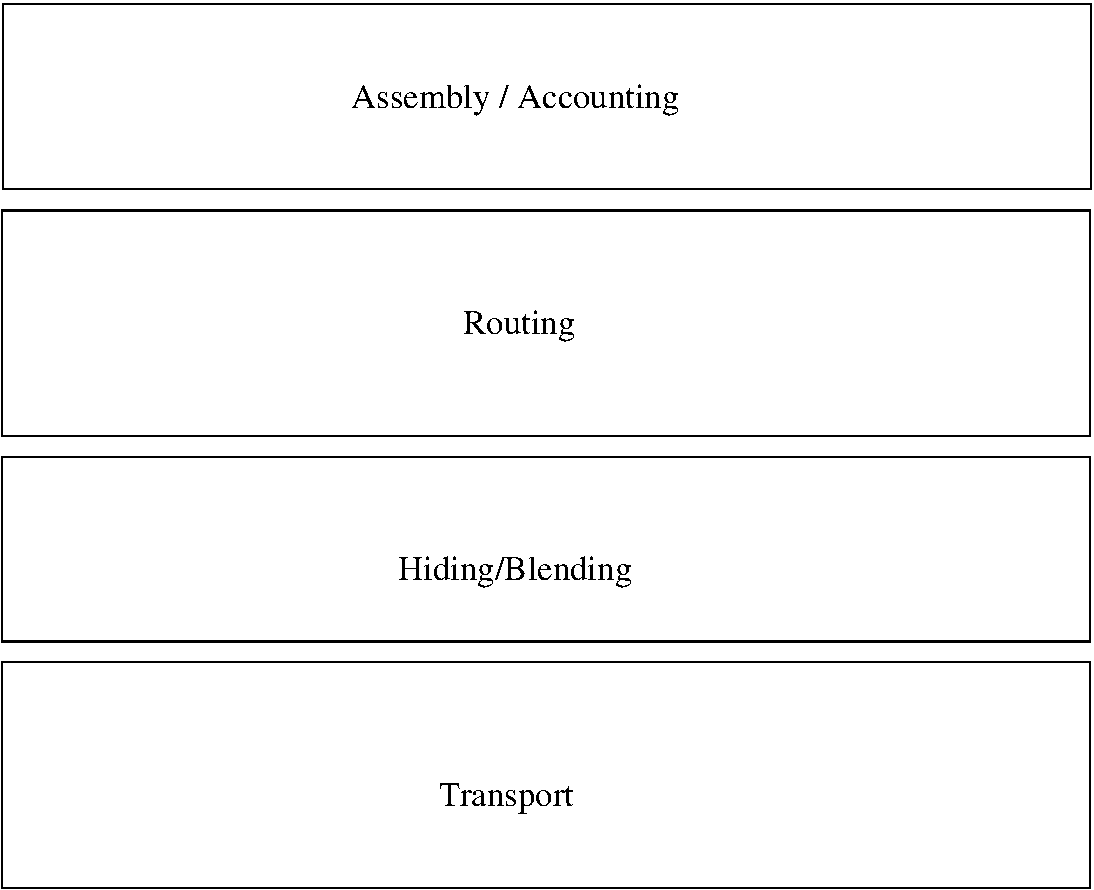
\includegraphics[width=\columnwidth]{inc/roughProtocolDesign}
	\caption{A first rough overview for the protocol}
	\label{fig:roughProtocolDesign}
\end{figure}	

The protocol itself should send messages through a well known transport protocol (``Transport'') which will be used for our messages. 

The messages will be hidden within regular messages already using that transport layer. In an ideal implementation messages sent by our protocol should be indistinguishable from regular messages (by computers and humans). In order to achieve this particular task we introduce a ``Hiding / Blending'' layer. This layer is normally specific to the underlying transport layer and may vary.

The ``Routing'' layer is the layer that receives and sends messages. It parses only the core protocol and the data processed here is completely independent from the underlying transport layer.

The ``Assembly / Accounting'' layer disassembles the received messages into its parts. It then recomposes and stores the messages for further routing. In order to avoid spaming over this media some kind of accounting will be involved. 

The messages passed through such a protocol stack are ononised to offer anonymity from evil nodes. Furthermore a node should be unable to tell whether a message was intended for a specific node or not (so all nodes including sender and recipient should handle identically).

In order to mitigate size based attacks (an onionised packet looses permanently data on its way) we introduce operations which may be applied to a valid message as well as to decoy traffic. The operations should be able to increase and decrease in size without being able to tell if this message is destined to a target or not. Operations not carried out due to missing data might be either intentionally or a malfunction.

The defined message operations are as follows:
\begin{itemize}
	\item Split a message block into two parts of variable size.\\
	      This operation may be used to fan out decoy traffic, to cut off decoy data, or to send multiple parts of a message through diffferent routing nodes.
	\item Join two data blocks to a bigger block using an xor operation.\\
	      This operation may be used to minimise decoy traffic or to rejoin data which has been split earlier.
	\item Fork off xor'ed data from a data block by applying an xor operation to a received block with a block of random data.\\
	      With this operation we may create decoy traffic, or split a message into two parts.
	\item Encrypt a block with a given key.      
	\item Decrypt a block with a given key.
\end{itemize}

To avoid making this system attractive to UBE an accounting system is introduced. The system works as follows:
\begin{itemize}
	\item Routing nodes may offer their services at a cost. These ``costs'' are typically paid by solving crypto puzzles.
	\item The following operations may be cost effective:
	\begin{itemize}
		\item Getting a discardable identity on a node (prerequisite for accounting).
		\item Allowance to route a number of messages through the node (cost per outgoing message) in a specified interval. This allowance is always linked to a discardable identity.
		\item Allowance to route a specific size of bytes through the node (cost per outgoing byte) in a specified time interval. This allowance is always linked to a discardable identity.
		\item Offer information about the known routing network by the node.
		\item Offer information about the identities current quota.
	\end{itemize}
\end{itemize}
All quotas require accounting. In order to minimise accounting all these quotas must be assigned a time interval in which they are effective. this guarantees that quota data is not growing indefinitely. It is up to the node to decide what time duration is still acceptable.

In order to limit the possibility to Denial of Service (DoS) a node by overloading it the following precautions are taken:
\begin{itemize}
	\item The message is built in such a way that message building is far more complex than message routing.
	\item Messages may be decrypted in parts to minimize the amount of work required to decide whether the full processing of the message will be done or the message is discarded anyway.
	\item The usage of inefficient operations (e.g. asymmetric encryption) is minimized.
	\item The server may limit specific operations.
\end{itemize}

\section{Rough Draft of Messages}
For our protocol we assume the following outline for a message:
\begin{itemize}
	\item Header block\\ 
	      This block contains an ephemeral identity of the sender on the message processing host. It allows the host to decide wether he is willing to process the rest of the message or not. It is important to know that the identity block contains a symmetric key for decryption of the main block and a secret repeated in the main block. This prevents that a malicious node may exchange the main block.
	\item Main block\\
	      This block contains all information regarding routing and processing data. It furthermore contains the payload data which may or may not contain messages.
	      \begin{itemize}
	      	\item Routing Blocks\\
	      	      This block contains information of which data block should be sent to what recipient. It furthermore may contain instruction for processing the data blocks and routing/reply blocks for subsequent processing. Another important thing to note is that routing blocks and payload data may arrive on two different paths to the target node.
	      	\item Routing Log Block\\
	      	      This Block contains information about the already occurred routing in onionised form. It may be regarded as the onionised pendant of received header in an SMTP header.
	      	\item Reply Block\\
	      	      This Block contains a Routing block which may be used to contact the original sender of a message (e.g. for an error message)
	      	\item payload Block\\
	      	      These Blocks form the payload data. It might contain a message, parts of a message or decoy material.
	      \end{itemize}      
\end{itemize}

The message is picked up from the transport layer and extracted in the blending layer. Processing is then split. First the Assembly/accounting layer is extracting the identity block and authorises further processing. The message building instructions are put into a identity specific list (with the expiration dates of the message). and the payload blocks are stored (again with the expiration date). 

After having prepared the message in such a way the routing layer gets the routing blocks. Every routing block is then processed after a final approval by the accounting layer (he is in charge to keep the quotas for this identity in  sync). The routing layer assembles the new messages according to the (no authorized) instructions in the routing block and sends it to the next hop where the processing restarts with the new instructions. 

\chapter{Existing Transport Layer Protocols}
In this chapter we have a look at various available transport layer protocol. The main goal is to identify strong candidates as a transport layer. Main focus lies on the following criterias:
\begin{itemize}
	\item Widely adopted (Ct1)\\
	      The more widely adopted and used a protocol is the harder it is for an adverser to monitor (due to the sheer mass), filter or block the protocol (censorship resistance).
	\item Reliable (Ct2)\\
	      Message transport between peers should be reliable. As messages may arrive anytime from everywhere we don not have means to synchronize the peer partners on a higher level without investing a considerable effort. In order to avoid this effort we do look for inherently reliable protocols.
	\item Symmetrical built (Ct3)\\
	      The transport layer should be built on a peer to peer base. All servers implement a generic routing which requires no prior knowledge of possible targets. This criteria neglects centralised infrastructures.
\end{itemize}

\section{HTTP}
The HTTP protocol allows message transfer from and to a server and is specified in RFC2616 \cite{RFC2616}. It is not suitable as a communication protocol for messages due to the lack of notifications. There are some extensions which would allow such communications (such as WebDAV) but in general even those are not suitable as they require a continous connection to the server in order to get notifications. Having a ``rollup'' of notifications when connecting is not there by default but could be implemented on top of it. 

HTTP servers listen on standard ports 80 or 443 for incomming connects. The port 443 is equivalent to the port 80 except for the fact that it has a wrapping encryption layer (usually TLS). The incomming connects (requests) must offer a header part and may contain a body part which would be suitable for transferring messages to the server. The reply onto this request is transferred over the same TCP connection containing the same two sections.

HTTP0.9-HTTP/1.1 are clear text protocols which are human readable (except for the data part which might contain binary data). The HTTP/2 (as specified in \cite{RFC7540}) is using the same ports and default behaviour. Unlike HTTP/0.9-HTTP/1.1 it is not a clear text but a binary protocol. Headers and bodies of messages are sent as binaries. 

The protocol does definitely satisfy the first two main criteria (Ct1: Widely Adopted and Ct2: Reliable).

The main disadvantage in terms as message transport protocol is that this protocol is not symetrically. This means that a server is always just ``serving requests'' and not sending actively information to peers. This Request-Reply violates criteria (Ct1: Symmetrically built) and makes the protocol not a primary choice for  message transport. 

\section{MQTT}
MQTT is an ISO standard (ISO/IEC PRF 20922:2016) and was formerly called MQ Telemetry Transport. The current standard as the time of writing this document was 3.1.1 \cite{mqtt}. 

The protocol runs by default on the two ports 1883 and 8883 and may be encrypted with TLS. MQTT is a publish/subscribe based message passing protocol which is mainly targeted to m2m communication. This Protocol requires the receiving party to be subscribed in a central infrastructure in order to be able to receive messages. This makes it very hard to be used in a system without centralistic infrastructure and having no static routes between senders and recipients.

The protocol does definitely satisfy the second criteria (Ct2: Reliable). It is in the area of enduser (i.e. Internet) not widely adopted thus violating Criteria 1 (Ct1: Widely Adopted). In terms of decentralistic design the protocol fails as well (Ct3: Symmetrically built).

\section{Advanced Message Queuing Protocol}
The Advanced Message Queuing Protocol (AMQP) was originally initiated by numerous exponents based mainly in finance related industries. The AMQP-Protocol is either used for communication between two message brokers, or between a message broker and a client\cite{amqp}.

It is designed to be interoperable, stable, reliable and safe. It supports either SASL or TLS secured communication. The usage of such a tunnel is controlled by the immediate sender of a message. In its current version 1.0 it does however not support a dynamic routing between brokers\cite{amqp}.

Due to the lack of a generic routing capability this protocol is therefore not suitable for message transport in a global generic environment.

The protocol satisfys partially the first criteria (Ct1: Widely Adopted), and fully satisfies the second criteria (Ct2: Reliable). However the third criteria is violated due to the lack of routing capabilities between message brokers (Ct3: Symmetrically built).

\section{Constrained Application Protocol (CoAP)}
The Constrained Application Protocol (CoAP) is a communication Protocol which is primarily destined to m2m communication. It is defined in RFC7252\cite{RFC7252}.  It is Defined as lightweight replacement for HTTP in IoT devices and is based on UDP.

The protocol does partially satisfy the first criteria (Ct1: Widely Adopted). The second criteria (Ct2: Reliable) is only partially fulfilled as it is based on UDP and does only add limited session control on its own.

The main disadvantage in terms as message transport protocol is that this protocol is not (like HTTP) symmetrically. This means that a server is always just ``serving requests'' and not sending actively information to peers. This Request-Reply violates criteria (Ct3: Symmetrically built) and makes the protocol not a primary choice for  message transport. 

\section{Web Application Messaging Protocol}
WAMP is a websockets based protocol destined to enable M2M communication. Like MQTT it is publish/subscribe oriented. Unlike MQTT it allows remote procedure calls (RPC).

The WAMP protocol is not widely adopted (Ct1: Widely Adopted) but it is definitely reliable on a per node base (Ct2: Reliable). Due to its RPC based capability unlike MQTT a routing like capability could be implemented. Symmetrical protocol behaviour is therefore not available but could be built in relatively easy.

\section{XMPP (jabber)}
XMPP (originally named Jabber) is a synchronous message protocol used in the internet. It is specified in the documents RFC6120\cite{RFC6120}, RFC6121\cite{RFC6120}, RFC3922\cite{RFC3922}, and RFC3923\cite{RFC3923}. The protocol is a very advanced chat protocol featuring numeros levels of security including end-to-end signing and object encryption\cite{RFC3923}. There is also a stream initiation extension for transferring files between endpoints \cite{xep0096}.

It has generic routing capabilities spanning between known and unknown servers.

The protocol itself seems to be a strong candidate as a transport layer as it is beeing used actively in the internet.

\fxfatal{figure out reliability of offline transfers and reliability in general}

\section{SMTP}
The SMTP protocol is currently specified in \cite{RFC5321}. It specifies a method to deliver reliably asynchronous mail objects thru a specific transport medium (most of the time the internet). The document splits a mail object into a mail envelope and its content. The envelope contains the routing information which is the sender (one) and the recipient (one or more) in 7-Bit ASCII. The envelope may additionally contain optional protocol extension material. \par

The content should be in 7-Bit-ASCII (8-Bit ASCII may be requested but this feature is not widely adopted). It is split into two parts. These parts are the header (which does contain meta information about the message such as subject, reply address or a comprehensive list of all recipients), and the body which contains the message itself. All lines of the content must be terminated with a CRLF and must not be longer than 998 characters excluding CRLF.\par

The header consists of a collection of header fields. Each of them is built by a header name, a colon and the data. Exact outline of the header is specified in \cite{RFC5322} and is separated with a blank line from the body. 

It \cite{RFC5321} furthermore introduces a simplistic model for smtp message based communication. A more comprehensive model is introduced in the section \nameref{sec:mailTransport}. As the proposed model is not sufficient for a comprehensive end-to-end analysis.\par

Traditionally the message itself is mime encoded. The MIME messages are mainly specified in \cite{RFC2045}, and \cite{RFC2046}. MIME allows to send messages in multiple representations (alternates), and attach additional information (such as possibly inlined images or attached documents). 

SMTP is one of the most common messaging protocols in the internet (Ct1: Widely Adopted) and it would be devastating for business of a country if for censoring reasons this protocol would be cut off. The protocol is furthermore very reliable as it has built in support for redundancy and a throughout message design making it relatively easy to diagnose problems (Ct2: Reliable). All SMTP servers are normally capable of routing and and receiving messages. Messages going over serveral servers are common (Ct3: Symmetrically built) so the third criteria may be considered as fulfilled as well

SMTP is considered a strong candidate as transport layer.  

\section{SMS}
SMS capability was introduced in the SS7 protocol. This protocol allows the message transfer of messages not bigger than 144 character. Due to this restriction in size it is unlikely to be suitable for this type of communication as the keys beeing required are already sized similarly leaving no space for Messages or routing information.

Secondly the protocol is not widely adopted within the internet domain. There are gateways providing bridging functionalities to the SMS service. However -- the protocol itself is insignificant in the internet itself. 

\fxfatal{add credible source}

\section{MMS}
The Multimedia Messaging Service (MMS) is maintained by 3GPP (\nth{3} Generation Partnership Project). This protocol is manly a mobile protocl based on telephone networks.

\fxfatal{analyse criterias and add more information}

\section{Roundup for Transport Protocols}
\begin{table}[h]
	\centering\tiny
	\begin{tabular}{|l|l|l|l|}\hline
		\diaghead{\theadfont protocol Criteria}{Protocol}{Criteria} & \thead{Ct1: Widely adopted} 	& \thead{Ct2: Reliable} & \thead{Ct3: Symmetrically built}\\\hline
		HTTP	 & $\checkmark$			& $\checkmark$		& $\times$\\              
		MQTT	 & \textasciitilde		& $\checkmark$		& $\times$\\              
		AMQP	 & \textasciitilde		& $\checkmark$		& $\times$\\
		CoAP	 & \textasciitilde		& \textasciitilde 	& $\times$\\
		WAMP	 & $\times$				& $\checkmark$		& \textasciitilde\\
		XMPP	 & $\checkmark$			& $\checkmark$		& $\checkmark$\\
		SMTP	 & $\checkmark$			& $\checkmark$		& $\checkmark$\\
		SMS\footnotemark[1] & 			& 					& \\
		MMS		 & $\checkmark$			& $\checkmark$		& $\times$\\\hline
	\end{tabular}	
	\caption{comparison of protocols in terms of the suitability criteria as transport layer}
	\label{tab:protoSuitCrit}
\end{table}

In table \ref{tab:protoSuitCrit} we sum up all previously analysed protocols. We use ``$\checkmark$'' for a fulfilled criteria, ``\textasciitilde'' for a partially fulfilled criteria, and ``$\times$'' for a not fulfilled criteria. This overview shows in compact form which protocols have been identified as strong candidates for use as a transport layer in terms of an anonymising protocol. 

This table shows that strong identified candidates are SMTP (being already a message sending protocol on asynchronous base) and XMPP (a real time chat protocol able to attach files. This protocol features furthermore end-to-end encryption and signing). Both have the advantages that they are really wide adopted in the internet and do support additionally advanced content (such as alternatives or attachments).

\footnotetext[1]{omitted due to message size being too small}


\chapter{Existing Research and Implementations on the Topic}
\section{Anonymity}
\DeclareFixedFootnote{\omitted}{footnotes omitted in quote}
As Anonymity we take the definition as specified in \cite{anon_terminology}.
\begin{quote}
	Anonymity of a subject means that the subject is not identifiable within a set of subjects, the anonymity set.\omitted
\end{quote}
and
\begin{quote}
	Anonymity of a subject from an attacker's perspective means that the attacker cannot sufficiently identify the subject within a set of subjects, the anonymity set.\omitted
\end{quote}

Whereas the anonymity set is defined as the set of all possible subjects.

Especially the anonymity of a subject from an attacker's is very important to this paper. 

\subsection{$k$-Anonymity}
$k$-anonymity is a term introduced in \cite{k-anonymous:ccs2003}. This work claims that no one might be held responsible for an action if the action itself can only be identified as an action which has been taken by one unidentifiable entity out of $k$ entities.

The Document distinguishes between \textit{Sender $k$-anonymity} where the sending entity can only be narrowed down to a set of $k$ entities and \textit{Receiver $k$-anonymity} 

\fxfatal{say something about the size of $k$; add more content}

\subsection{$\ell$-Diversity}
In \cite{machanavajjhala2007diversity} an extended model of $k$-anonymity is introduced. In this paper the the authors emphasize that it is possible to break a $k$-anonymity set if there is additional Information available which may be merged into a data set so that a special entity can be filtered from the $k$-anonymity set. In other words if an anonymity set is to tightly specified a single additional background information might be sufficient to identify a specific entity in an anonymity set.

While it might be arguable that a $k$-anonymity in which a member is not implicitely $k$-anonymous still is sufficient for $k$-anonymity in its sense the point made in this work is definitely right and should be taken into account.

Their approach is to introduce an amount of invisible diversity into $k$-anonymous sets so that simple background knowledge is no longer sufficient to isolate a single member.

\subsection{$t$-Closeness}
While $\ell$-diversity protects the identity of an entity it does not prevent information gain. A subject which is in a class has the same attributes. This is where $t$-closeness\cite{li2007t} comes into play. $t$-closeness is defined as follows:

\begin{quote}
  An equivalence class is said to have $t$-closeness if the distance between the distribution of a sensitive attribute in this class and the distribution of the attribute in the whole table is no more than a threshold. A table is said to have $t$-closeness if all equivalence classes have $t$-closeness.
\end{quote}

\section{Zero Trust}
Zero trust is not a truly researched model in systems engineering. It is however widely adopted. 

We refer in this work to the zero trust model when denying the trust in any infrastructure not directly controlled by the sending or receiving entity. This distrust extends especially but not exclusively to the network transporting the message, the nodes storing and forwarding messages, the backup taken from any system except the client machines of the sending and receiving parties, and software, hardware, and operators of all systems not explicitly trusted.

As explicitely trusted in our model we do regard the user sending a message (and his immediate hardware used for sending the message), and the users receiving the messages. Trust in between the receiving parties (if more than one) of a message is not necessarily given.

\section{Pseudonymity}
As Pseudonymity we take the definition as specified in \cite{anon_terminology}.

\begin{quote}
	A pseudonym is an identifier of a subject other than one of the subject's real
	names. The subject which the pseudonym refers to is the holder of the pseudonym. A subject is pseudonymous if a pseudonym is used as identifier instead of one of its real names.\omitted
\end{quote}

\section{Undetectability}
As undetectability we take the definition as specified in \cite{anon_terminology}.

\begin{quote}
	Undetectability of an item of interest (IOI\index{Item of Interest}) from an attacker's perspective means that the
	attacker cannot sufficiently distinguish whether it exists or not.\omitted
\end{quote}

\section{Unobservability}
As unobservability we take the definition as specified in \cite{anon_terminology}.

\begin{quote}
	Unobservability of an item of interest (IOI) means
	\begin{itemize}
		\item undetectability of the IOI against all subjects uninvolved in it and
     	\item anonymity of the subject(s) involved in the IOI even against the other subject(s) involved in that IOI.
	\end{itemize}
	
\end{quote}

This part is very important. As we are heading for a censorship resistant solution unobservability is a key. As mentioned in this paper unobservability raises the bar of required attributes again ($\Rightarrow$ reads ``implies''):
\begin{eqnarray*}
	censorship\ resistance & \Rightarrow & unobservability\\
	unobserability         & \Rightarrow & undetectability\\
	unobserability         & \Rightarrow & anonymity
\end{eqnarray*}

So this means that we have to use an undetectable data channel in order to achieve censorship resistance.

\subsection{Ephemeral Identity}
In this work we use accounting on various levels. While we are dealing with anonymity accounting has still to be linked to some kind of identity for this reason we are introducing a term called ``ephemeral identity''.

\begin{quote}
	A Ephemeral identity is a temporary identity which is defined by the following attributes:
	\begin{itemize}
		\item It is an artificial identity
		\item It is only used for a short timespan
		\item It is not linkable to another identity
	\end{itemize}
\end{quote}

The key in this definition is the last point is crucial and at the same time hard to achieve.

\section{Single Use Reply Blocks and Multi Use Reply Blocks}
The use of single use reply blocks were first introduced by Chaum in \cite{CHAUM1}. A routing block in general is a structure allowing to send a message to someone without knowing the targets true address. It might be differentiated into ``Single Use Reply Bolcks'' (\defref{SURB}s) which may be used once and ``Multi Use Reply Blocks'' (\defref{MURB}s) which may be used a limited number of times. 

The concept is that we have in our case a routing block which might be used up to $n$ times ($0<n<127$). The number has been chosen for practical reasons. It is easily representable in a byte integer (signed or unsigned) on any system. It is big enough to support human communication in a sensible way and is big enough to add not too much overhead when rerequesting more \defref{MURB}s. The number should not be too big because if a \defref{MURB} is reused the same pattern of traffic is generated thus making the system susceptible to statistical attacks.

\section{Censorship}
As definition for censorship we take
\begin{quote}
	Censorship: the cyclical suppression, banning, expurgation, or editing by an individual, institution, group or government that enforce or influence its decision against members of the public -- of any written or pictorial materials which that individual, institution, group or government deems obscene and "utterly without redeeming social value," as determined by "contemporary community standards.".
\end{quote}
Which is attributed to Chuck Stone Professor at the School of Journalism and Mass Communication, University of North Carolina. Please note that ``Self Censorship'' (not expressing something in fear of consequences) is a form of censorship too.

In our more technical subsystem this means
\begin{quote}
	A systematic suppression, modification, or banning of data in the internet by either removal, or modification of the data, or systematic influencing of entities involved in the processing (e.g. by writing, routing, storing or reading) of this data.
\end{quote}

\subsection{Censorship Resistant}
A censorship resistant system is a system which allows the users of the system and the data itself to be unaffected from censorship. Please note that this does not deny the possibility of censorship per se. It still exists outside the system. But it has some consequences for the system itself.

\begin{itemize}
	\item The system must be either undetectable or out of reach for an entity censoring.\\
	      The possibility of identifying a protocol or data allows a censoring entity to suppress the use of the protocol itself. 
	\item The entities involved in a system must be untraceable.\\
	      Traceable entities would result in means of suppressing real world entities participating in the system.
\end{itemize}

\subsection{Parrot Circumvention}
In \cite{oakland2013-parrot} \citeauthor{oakland2013-parrot} express that it is easy for a human to determine decoy traffic as the content is easily identifiable as automated content. While this is absolutely true there is a possibility here to generate ``human like'' data traffic to a certain extent. In our design this is the job covered by the blending layer.

\subsection{Censorship Circumvention}
Several technical ways have been explored to circumvent censorship. All seem to boil down to two main ideas:
\begin{itemize}
	\item Hide data.
	\item Copy data to a vast amount of places in order to improve the lifespan of data.
\end{itemize}

In the following section we look at technologies and ideas dealing with these circumvention technologies.

\subsubsection{Covert Channel}
\fxfatal{add content here}

\subsubsection{Spread Spectrum}
\fxfatal{add content here}

\section{Cryptography}
Whenever dealing with hiding data and maintaining integrity of data cryptography is the first tool in the hand of an implementer. A vast amount of research in this area does already exist. For this work we did not collect a lot of information. We focussed on algorithms either well researched and implemented or research which seem very valuable when putting this work into place. 

\subsection{Symmetric Encryption}
Symmetric encryption in this paper assumes always that
\begin{eqnarray}
D^{K_a}\left(E^{K_a}\left(M\right)\right) & = & M
\end{eqnarray} 

For a key $K_b\neq K_a$ this means
\begin{eqnarray}
D^{K_a}\left(E^{K_b}\left(M\right)\right) & \neq & M\\
D^{K_b}\left(E^{K_a}\left(M\right)\right) & \neq & M
\end{eqnarray} 

\subsubsection{AES}
\fxfatal{add content here}

\subsection{Asymmetric Encryption}
For all asymmetric encryption algorithm in this paper we may assume that 
\begin{eqnarray}
D^{K^{-1}_a}\left(E^{K^{1}_a}\left(M\right)\right) & = & M\\
D^{K^{1}_a}\left(E^{K^{-1}_a}\left(M\right)\right) & = & M
\end{eqnarray} 

It is important that 
\begin{eqnarray}
D^{K^{-1}_a}\left(E^{K^{-1}_a}\left(M\right)\right) & \neq & M\\
D^{K^{1}_a}\left(E^{K^{1}_a}\left(M\right)\right) & \neq & M
\end{eqnarray} 

And for any other Keypair $K^{p}_a \neq K^{p}_b$
\begin{eqnarray}
D^{K^{-1}_b}\left(E^{K^{1}_a}\left(M\right)\right) & \neq & M\\
D^{K^{1}_b}\left(E^{K^{1}_a}\left(M\right)\right) & \neq & M\\
D^{K^{-1}_b}\left(E^{K^{-1}_a}\left(M\right)\right) & \neq & M\\
D^{K^{1}_b}\left(E^{K^{-1}_a}\left(M\right)\right) & \neq & M
\end{eqnarray} 

\subsubsection{RSA}
In \citeyear{Rivest:1978:MOD:359340.359342} the authors \citeauthor{Rivest:1978:MOD:359340.359342} published with \cite{Rivest:1978:MOD:359340.359342} a paper which did revolutionize cryptography for years. In their paper the authors described an encryption method later to be called RSA which required a key pair ($K_a$) referenced as public ($K^{1}_a$) and private keys ($K^{-1}_a$). The novelty of this system was that anything encrypted with the public key was only decryptable with the private key and vice versa.

RSA is up until the day of writing this paper not publicly know to be broken (unless a too small key size is used). However -- \citeauthor{Shor97polynomial-timealgorithms} described in \citeyear{Shor97polynomial-timealgorithms} an algorithm which should enable quantum computers to break RSA far faster than done with common computers. In the section \ref{sec:keySize} we do elaborate this effects further.

\subsubsection{Elliptic Curve Cryptogaphy}
The elliptic curves were independently suggestd by \cite{Miller1986} and \cite{Koblitz04guideto} in 1986. Elliptic curve Cryptography started to be widely deployed in the public space about in 2006. Since then it seems to compete very well with the well established RSA algorithm. While being similarly well researched ECC has the advantage of far shorter key sizes for the same grade of security.

\subsection{Homomorphic encryption}
\fxfatal{add content here}

\subsection{Deniable Encryption and Deniable Steganography}
\fxfatal{add content here}

\subsection{Key Sizes\label{sec:keySize}}
The question of key sizes is a hard to answer as it depends on the current and future possibilities of an adverser which is again depending on not forseeable research. We tried to collect a couple of recommendatitions.

\href{http://www.ecrypt.eu.org/}{Encrypt II (http://www.ecrypt.eu.org/)} recommends currently for a ``forseeable future'' 256 Bits for symmetric encryption and for asymmetric encryption based on factoring modulus 15424 Bits. Elliptic Curve Cryptography and Hashing should be sufficient if used with at least 512 Bits. If the focus is reduced to the next $\approx$ 20 years then the key size recommendations is reduced to 128 Bit for symmetric encryption, 3248 Bits for factoring modulus operations and 256 Bits for elliptic curves and hashing.

According to the equations proposed by \citeauthor{Lenstra04keylength.} in \cite{Lenstra04keylength.} an asymmetric key size of 2644 Bits respectively a symmetric key length of 95 Bits, or 190 Bits for elliptic curves and hashing should be sufficient for security up to the year 2048. 

According to \cite{nsa-fact-sheet-B} data classified up to ``top secret'' should be secured asymmetric encryption based on factoring modulus (no proposed encryption standard).  For symmetric encryption they recommend 256 Bits, for Hashing at least SHA-384 and for Elliptic curves a 384 Bit sized key.

As it might seem not a wise idea to consider the recommendation of a potential state sponsored adverser and the Formulas proposed by \citeauthor{Lenstra04keylength.} do not explicitly take quantum computers into account we therefore follow the recommendations of ENCRYPT II.

Furthermore taking all recommendations together it seems that all involved parties assume the biggest trust into elliptic curves rather than asymmetric encryption based on factoring modulus.

\section{Routing}
If we can follow data from a source to a destination we may safely assume that the participants of this data exchange are no longer anonymous. So special care should be taken to this aspect. In the past several approaches have been made in order to avoid detection of data while routing. in the following sections we will look at some basic concepts which have been proposed up until today. We describe their concept and have a look at their weaknesses discovered so far.

In \nameref{sec:sysImpl} we the analyze some related real world systems regarding how they work and how they have been attacked in the past.

\subsection{Mixing}
Mixes have been first introduced by \citetitle{CHAUM1}\cite{CHAUM1} in \citeyear{CHAUM1}. The basic concept in a mix goes as follows. We do not send a message directly from the source to the target. Instead we use a kind of proxy server or router in between which picks up the packet, anonymizes it, and forwards it either to the recipient or another mix. If we assume that we have at least 3 mixes cascaded we then can conclude that:
\begin{itemize}
	\item Only the first mix knows the true sender
	\item All intermediate mixes know neither the true sender nor the true recipient (as the data comes from mixes and is forwarded to other mixes) 
	\item Only the last mix knows the final recipient.
\end{itemize}

This approach (in this simple form) has several downsides and weaknesses.

\begin{itemize}
	\item In a low latency network the message may be traced by analysing the timing of a message.
	\item We can emphasize a path by replaying the same message multiple times (assuming we control an evil node) thus discovering at least the final recipient.
	\item If we can ``tag'' a message (with a content or an attribute) we then may be able to follow the message.
\end{itemize}

In \citeyear{RP03-1} \citeauthor{RP03-1} analyzed the suitability for mixes as a anonymizing network for masses. They concluded that there are three possibilities to run mixes.
\begin{itemize}
	\item Commercial Static MixNetworks
	\item Static MixNetworks Operated by Volunteers
	\item Dynamic MixNetworks
\end{itemize}
They concluded that in an ideal implementation a dynamic mix network where every user is operating a mix is the most promising solution as static mixes always might be hunted by an adverser.

\subsection{Onion Routing}
Onion routing is a further development of the concept of mixes. In onion routers every mix gets a message which is asymmetrically encrypted. By decrypting the message he gets the name of the next hop and the content which he has to forward. The main difference in this approach is that in traditional mix cascades the mix decides about the next hop. In an onionised routing system the message decides about the route it is taking. 

While tagging attacks are far harder (if we exclude side channel attacks to break sender anonymity) the traditional attacks on mixes are still possible. So when adversers are operating entry and/or exit nodes it is very easy for them to match the respective traffic.

One very well known of onion routing networks is Tor (\href{https://www.torproject.org}{https://www.torproject.org}). For more information about tor see section \ref{sec:tor}.

\fxfatal{\cite{onion-routing:pet2000}; Add reference that onion routers work "Connection based"}

\subsection{Crowds}
Crowds is a network which offers anonymity within a local group. It works as follows:
\begin{itemize}
	\item All users add themselfes to a group by registering on a so called ``blender''.
	\item All users start a service (called jondo).
	\item Every Johndo takes any received message (might be from him as well) and sends it with a 50\% chance either to the correct recipient or to a randomly chosen destination
\end{itemize}
While crowds do anonymize the sender from the recipient rather well the system offers no protection from someone capable of monitoring crowds traffic. The system may however be easily attacked from within by introducing collaborating jondos.

\fxfatal{suspectible to timing analysis; mention example Freenet; \cite{crowds:tissec};\cite{DBLP:conf/esorics/DanezisDKT09}}

\subsection{Mimic routes}
Mimics are a set of statical mixes which maintain a constant message flow between the static routes. If legitimate traffic arrives the pseudo traffic is replaced by the legitimate traffic an outstanding observer is thus incapable of telling the difference between real traffic and dummy traffic.

If centralized mixes are used the system lacks the same vulnerabilities of sizing and observing the exit nodes as all previously mentioned systems. If we assume that sender and receiver operate a mixer by themselves the system would be no longer susceptible to timing or sizing analyses. The mimic routes put a constant load onto the network. This bandwidth is lost and may not be reclaimed. It does not scale well as every new participant increases the need for mimic routes and creates (in the case of user mixes) new mimic load.

\subsubsection{DC Networks}
DC networks are based on the work \citetitle{chaum-dc} by \citeauthor{chaum-dc}\cite{chaum-dc}. In this work \citeauthor{chaum-dc} describes a system allowing a one bit transfer (The specific paper talks about the payment of a meal). Although all participants of the DC net are known the system makes it unable to determine who has been sending a message. The message in a DC-Net is readable for anyone. This network has the downside that a cheating player may disrupt communication without being traceable.

Several attempts have been made to strengthen the proposal of Chaum\cite{golle:eurocrypt2004}\cite{disco}. But no one succeeded without introducing significant downsides on the privacy side.

\subsubsection{Annonymous Remailer\label{sec:remailer}}
Remailers have been in use for quite some time. There are serveral classes of remailers and all of them are somehow related to Mixnets. There are ``types'' of remailers defined. Although these ``types'' offer some kind of hierarchy none of the more advanced ``types'' seem to have more than one implementation in the wild. \fxfatal{verify again if this claim is true}

Pseudonymous Remailers (also called Nym Servers) take a message and replace all information pointing to the original sender with a pseudonym. This pseudonym may be used as an answer address. The most well known psydonymous remailer possibly was anon.penet.fi run by Johan Helsingius. This service has been forced several times to reveal a pseudonyms true identity before Johan Heösingius decided to shut it down. For a more in depth discussion of Pseudonymous Remailers see \ref{sec:remPsydo}

Cypherpunk remailers forward messages like pseudonymous remailers. Unlike pseudonymous remailers Cypherpunk remailers decrypt a received message and its content is forwarded without adding a pseudonym. A reply to such a message is not possible. They may therefore be regarded as an ``decrypting reflector'' or a ``decrypting mix'' and may be used to build an onion routing network for messages. For a more in depth discussion of Type I Remailers see \ref{sec:remCypherpunk}.

Mixmaster remailers are very similar to Cypherpunk remailers. Unlike them Mixmaster remailers hide the messages not in an own protocol but use SMTP instead for it. While using SMTP as a transport layer Cypherpunk remailers are custom (non traditional mail) servers listening on port 25. For a more in depth discussion of type II remailers see \ref{sec:remMixmaster}.

Mixminion remailers extend the model of Mixmaster remailers. They still use SMTP but introduce new concepts. New concepts in Mixminion remailers are:
\begin{itemize}
	\item Single Use Reply Blocks (SURBs)
	\item Replay prevention
	\item Key rotation
	\item Exit poicies
	\item Dummy traffic
\end{itemize}
For a more in depth discussion of Mixminion remailers see \ref{sec:remMixminion}.

\fxfatal{add citations here; be more precise as remailer are somehow related to our solution}

\subsection{Cryptopuzzles}
\fxfatal{Cryptopuzzles from "Theoretical and experimental methods for defending against DDOS attacks" by Mohammad Reza Khalifeh Solta}

\subsubsection{Argon2}
\fxfatal{add Argon2 (memory hard)}

\section{System Implementations\label{sec:sysImpl}}
The following sections emphasize on implementations of anonymising (and related) protocols regardless of their usage in the domain of messaging. It is a list of system classes or their specific implementations together with a short analysis of strength and weaknesses. Wherever possible we try to refer to original sources. This is however not always possible since some of these systems are no longer in use.

If a system shows strong similarities in parts then we emphasize on this parts and analyse the findings.

\subsection{Pseudonymous Remailer\label{sec:remPseudo}}
The basic idea of remailers were dicussed in \cite{CHAUM1}. The most well known remailer was probably anon.penet.fi which operated from 1993 to 1996. 

In principle an anonymous remailer works as an ordinary forwarding SMTP server. The only difference is that it strips off all header fields except for ``from'', ``to'', and ``subject'' and then replaces the sender and recipient address with pseudonyms (if any). 

As the example shows this kind of remailer is easily attackable by an authority. Since the remailer knows tuples of pseudonyms and their respective real identity it may be forced to reveal true identities. Furthermore message may be monitored at the server or on its way and then due to the content a matching or even tagging is possible.

This remailer offers therefore no protection against an adverser defined in our problem.

\subsection{$I^2P$}
\fxfatal{add content here}

\subsection{Babel}
Babel was an academic system defined in a paper by \citeauthor{babel} in \citeyear{babel}\cite{babel}.
\fxfatal{add content here}

\subsection{Cypherpunk-Remailer\label{sec:remCypherpunk}}
\fxfatal{add content here}

\subsection{Mixmaster-Remailer\label{sec:remMixmaster}}
\fxfatal{add content here}

\subsection{Mixminion-Remailer\label{sec:remMixminion}}
\fxfatal{add content here}

\subsection{Crowds}
\fxfatal{add content here}

\subsection{Tarzan}
\fxfatal{add content here}

\subsection{Tor\label{sec:tor}}
\fxfatal{add content here}

\subsection{Herbivore}
\fxfatal{add content here}

\subsection{Dissent}
\fxfatal{add content here}

\subsection{P5}
\fxfatal{add content here}

\subsection{Gnutella}
\fxfatal{add content here}

\subsection{Gnutella2}
\fxfatal{add content here}

\subsection{Freenet}
\fxfatal{add content here}

\subsection{Darknet}
\fxfatal{add content here}

\subsection{Sneakernet}
\fxfatal{add content here}

\subsection{Hordes}
\fxfatal{add content here}

\subsection{Salsa}
\fxfatal{add content here}

\subsection{Hydra-Onion}
\fxfatal{add content here}

\subsection{SMTP}
As SMTP is our trasport prototype we focus in depth onto this topic.

Todays mail transport is mostly done via SMTP\index{SMTP} protocol as specified in \cite{RFC5321}. This protocol has proven to be stable and reliable. Most of the messages are passed from a MUA to a SMTP relay of a provider. From there the message is directly sent to the SMTP server of the recipient and from there to a server based storage of the recipient. The recipient may at any time connect to his server based storage and may optionally relocate the message to a client based (local) storage. The delivery from the server storage to the MUA of the recipient may happen by message polling or by message push (where as the later is usually implemented by a push-pull mechanism).\par

To understand the routing of a mail it is essential to understand the whole chain starting from a user(-agent) until arriving at the target user (and being read!). To simplify this I used a consistent model which includes all components (server and clients). The figure \ref{fig:MailAgents} shows all involved parties of a typical Mail routing. It is important to understand that Mail routing remains the same regardless of the used client. However -- Availability of a mail at its destination changes drastically depending on the type of client used. Furthermore control of the mail flow and control is different depending on the client.\par

The model has three main players storage (derfref{Storage}), agent (derfref{Agent}) and service (derfref{Service}). Storages are endpoint storages storing mails. Not explicitely shown are temporary storages such as spooler queues or state storages. Agents are simple programs taking care of a specific job. Agents may be exchangeable by other similar agents. A service is a bundle of agents which is responsible for a specific task or task sets.

\begin{figure}[ht!]
	\centering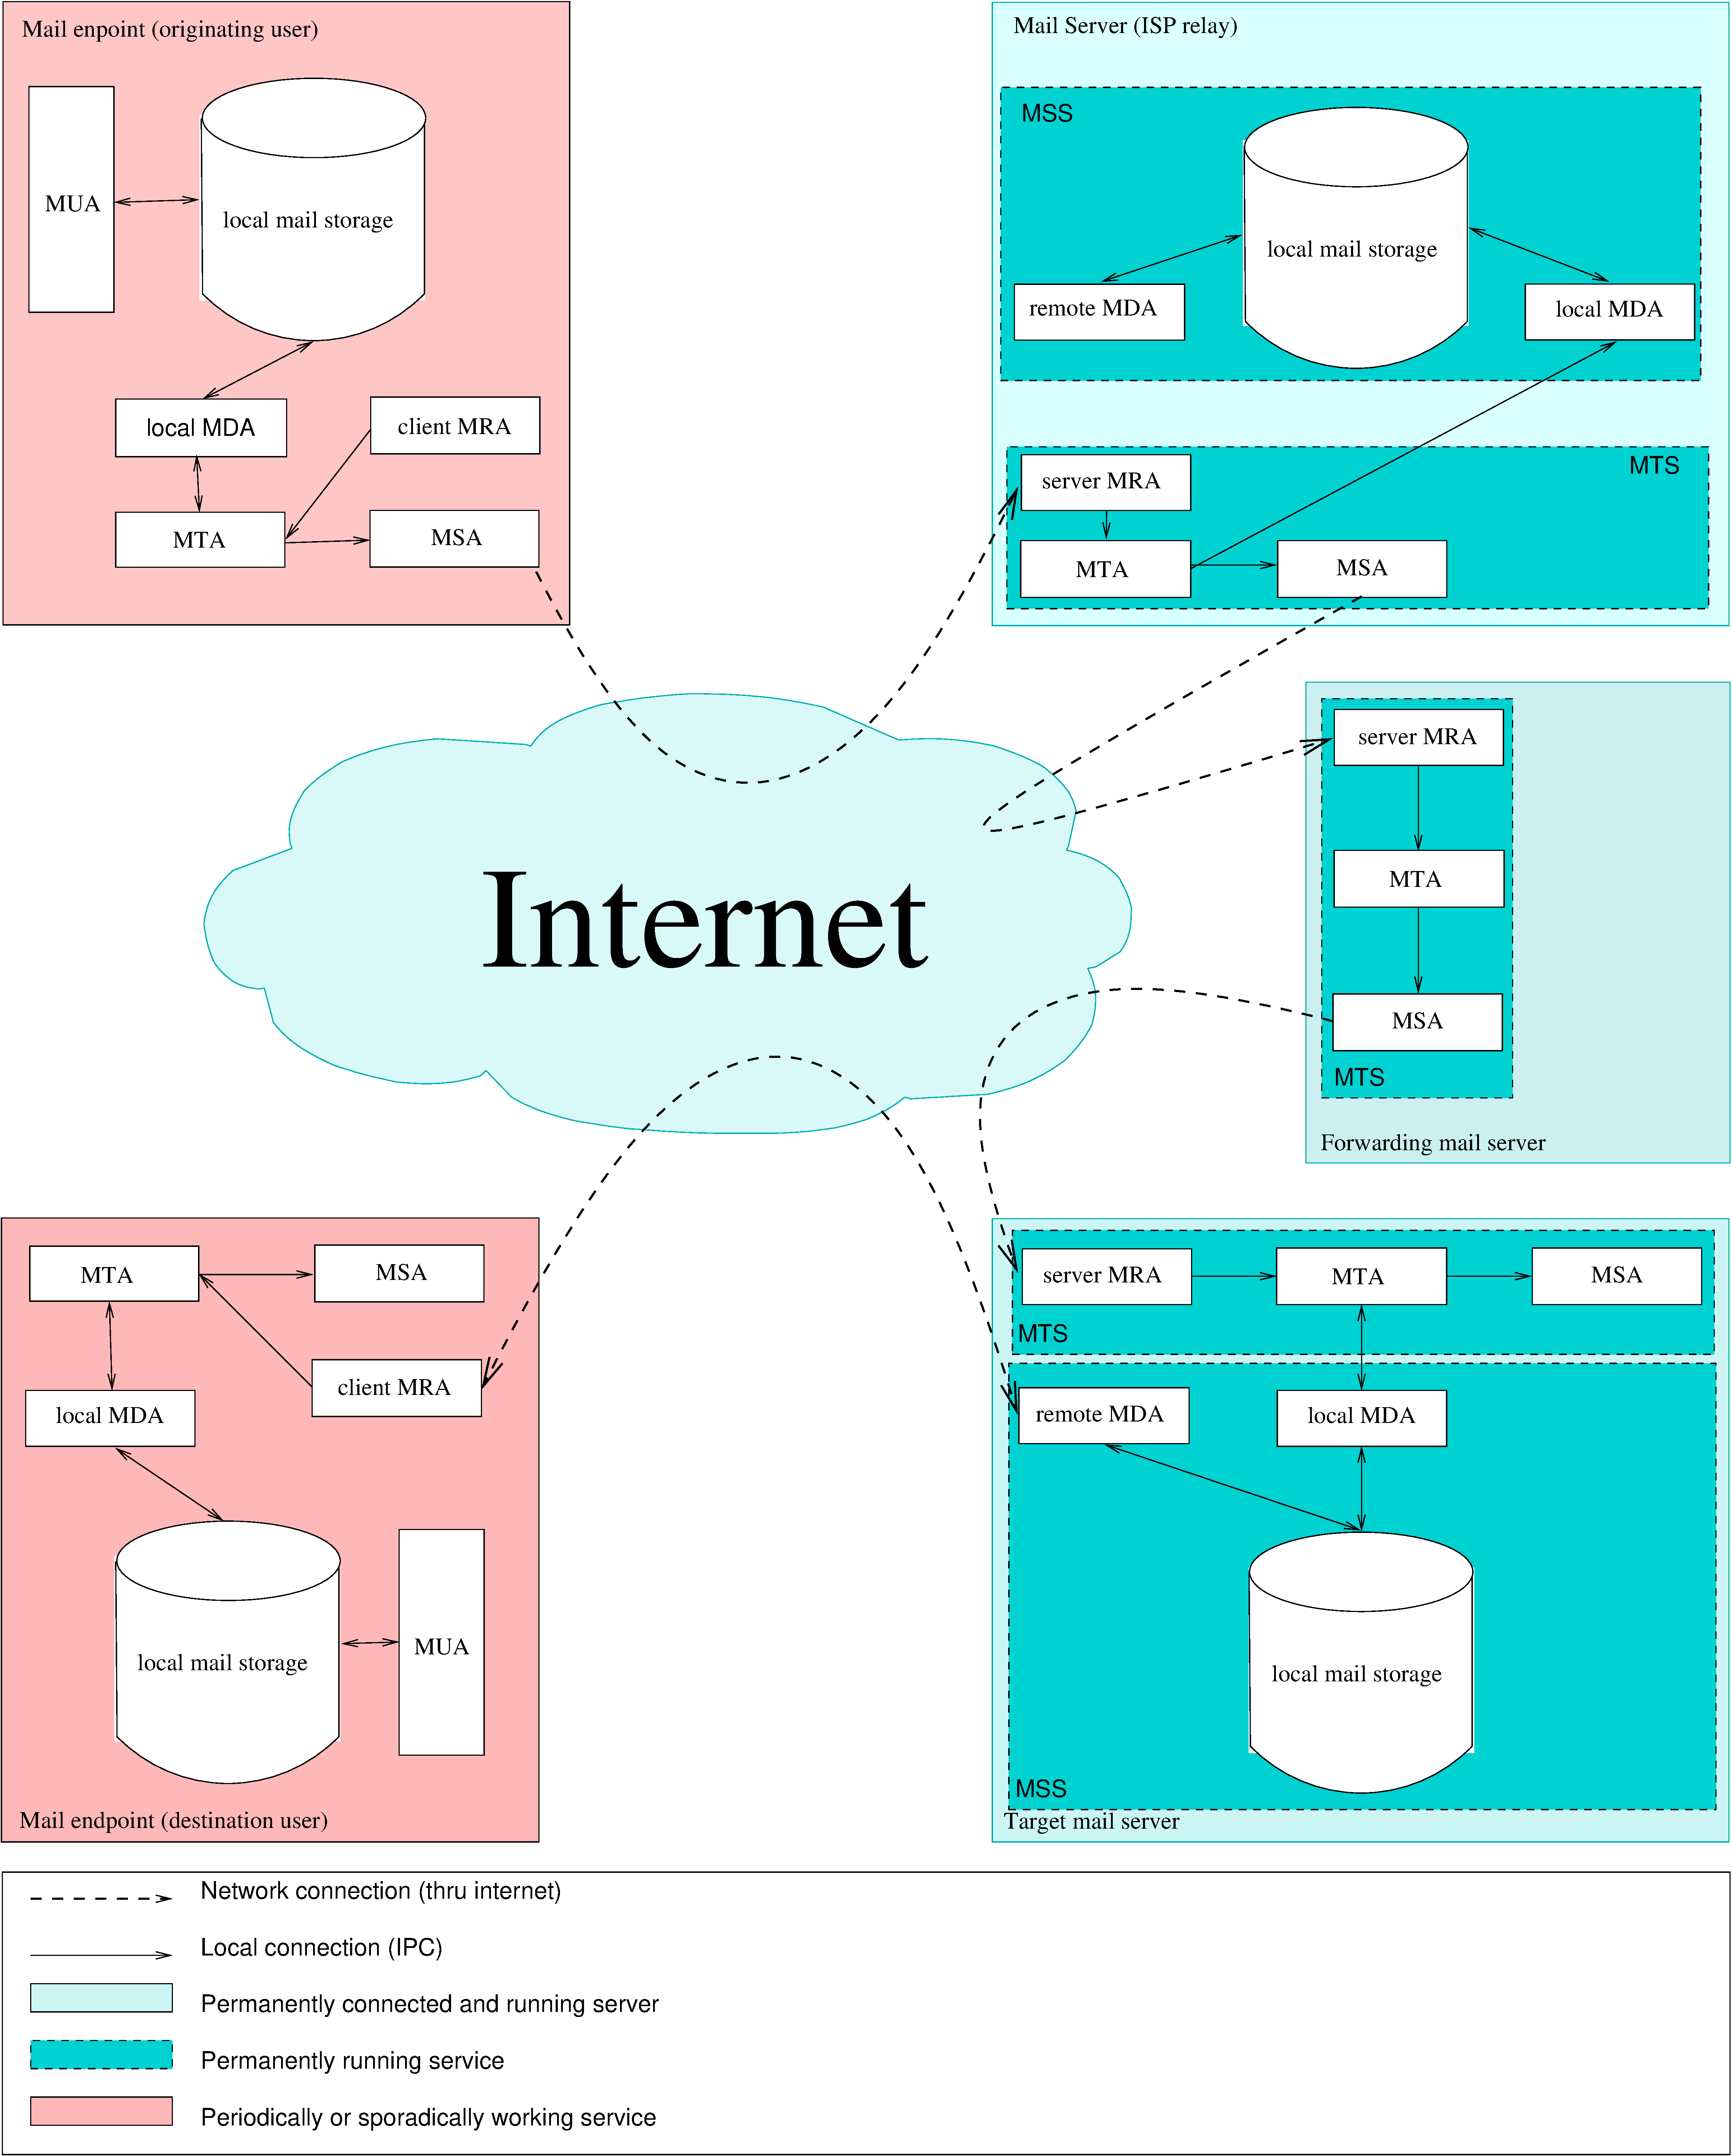
\includegraphics[width=\columnwidth]{inc/MailAgents1.pdf}
	\caption{Mail Agents}\label{fig:MailAgents}
\end{figure}

In the following paragraphs (for definitions) the term ``Mail'' is used synonymously to the term ``Message''. The reason why ``Mail'' has been chosen over ``Messages'' that a lot of terms do already exist in standard documents. In these documents the term mail is commonly used.\par

Mails are typically initiated by a Mail User Agent (\defref{MUA}). A MUA accesses a local mail storage which may be the server storage or a local copy. The local copy may be a cache only copy, the only existing storage (when mails are fetched and deleted from the server after retrieval) or a collected representation of multiple server storages (cache or authoritative).\par

Besides the MUA the only other component accessing a local mail storage is the Mail Delivery Agent (\defref{MDA}). An MDA is responsible for storing and fetching mails from the local mail storage. Mails destined for other accounts than the current one are forwarded to the MTA. Mails destined to a User are persistently stored  in the local mailstorage. It is important to understand that a mailstorage not nessesarily reflects a simple mailbox. It may as well represent multiple mailboxes (eg. a rich client serving multiple IMAP accounts) or a combined view of multiple accounts (eg. a rich client collecting mail from multiple \defref{POP} accounts. In the case of a rich client the local MDA is part of the software provided by the user agent. In the case of a mail server the local MDA is part of the local Mailstore (not necessarily of the mail transport service).

On the server side there are usually two components (services) at work. A ``Mail Transport Service'' (\defref{MTS}) responsible for mail transfers and a ``Mail Storage System'' which offers the possibility to store received Mails in a local, persistent store.\par

A MTS consists generally out of three parts. For incoming connects there is a daemon called Mail Receiving Agent (\defref{Server MRA}) is typically a \defref{SMTP} listening daemon. A Mail Transfer Agent (\defref{MTA}) which is responsible for routing, forwarding and rewriting mails. And a Mail Sending Agent (\defref{MSA}) which is responsible for transmitting mails reliably to another Server MRA (usually sent via \defref{SMTP}).\par

A MSS consists out of a local storage and delivery agents which do offer uniform interfaces to access the local store. They do also deal with replication issues and grant should take care of the atomicity of transactions committed to the storage. Typically there are two different kind of \defref{MDA}s. \defref{Local MDA}s offer possibilities to access the store via efficient (non network based) mechanisms (eg IPC or named sockets). This is usually done with a stripped down protocol (eg. \defref{LMTP}). For remote agents there a publicly -- network based -- agent available. Common Protocols for this \defref{Remote MDA}\ include \defref{POP}, \defref{IMAP}, or \defref{MS-OXMAPIHTTP}.\par

\subsection{Mail Endpoints}
Mail endpoints consist typically of the following components:
\begin{itemize}
	\item A Mail User agent (\defref{MUA})
	\item A Local Mail storage (\defref{MUA})
	\item A Local Mail Delivery Agent (\defref{Local MDA})
	\item A Mail Transfer Agent (\defref{MTA})
	\item A Mail Sending Agent (\defref{MSA})
	\item A Mail Receiving Agent (\defref{MRA})
\end{itemize}

Only two of these components do have external interfaces. These are \defref{MSA} and \defref{MRA}. \defref{MSA} usually uses \defref{SMTP} as transport protocol. When doing so there are a couple of specialities. 
\begin{itemize}
	\item Portnumber is 587 (specified in \cite{RFC4409}).\\
	Allthough port numbers 25 and 465 are valid and do have usually the same capabilities, they are for mail routing between servers only. Mail endpoints should no longer use them.
	\item Connections are authenticated.\\
	Unlike a normal server-to-server (relay or final delivery) SMTP connections on port 25 clients should always be authenticated of some sort. This may be based on data provided by the user (eg. username/passsword or certificate) or data identifying the sending system (eg. IP address)\cite{RFC4409}. Failure in doing authentication may result in this port beeing misused as an sender for \defref{UBE}.
\end{itemize}

Mail User Agents (MUA) are the terminal endpoint of a mail delivery. Mail user agents may be implemented as fat clients on a desktop or mobile system or as an interface over a different generic protocol such as HTTP (Web Clients). \par

Server located clients are a special breed of fat clients. These clients share the properties of fat clients except for the fact that they do not connect to the server. The client application itself has to be run on the server where the mail storage persists. This makes delivery and communication with the server different. Instead of interfacing with a MSA and a client MDA they may directly access the local mail storage on the server. On these systems the local mail storage may be implemented as a database in a user specific directory structure.

\subsubsection{Fat clients}
The majority of mail clients are fat clients. These clients score over the more centralistic organized web clients in the way that they may offer mail availability even if an internet connection is not available (thru a client specific local mail storage). They furthermore provide the possibility to collect mails from multiple sources and store them in the local storage. Unlike Mail servers, clients are assumed to be not always online. In fact they may be offline most of the time. To guarantee the availability of a certain email address a responsible mail server for a specific address collects all mails (this is done by the \defref{MSS}) and provides a consolidated view onto the database when a client connects thru a local or remote MDA.\par

As these clients vary strongly it is absolutely mandatory for the MDA that they are well specified. Lack in doing so would result in heavy interoperability problems. Most commonly the Protocols \defref{IMAP}, \defref{POP} and \defref{EWS} are being used these days. For mail delivery the SMTP protocol is used. \par

Fat clients ar comonly used on mobile devices. According to  \cite{clientDistribution} in Aug 2012 the most common fat email client was Apple Mail client on iOS devices ($35.6\%$), followed by Outlook ($20.14\%$), and Apple Mail ($11\%$). \citetitle{clientDistribution2}\cite{clientDistribution2} as a more recent source lists in February 2014 iOS devices with $37\%$, followed by Outlook ($13\%$), and  Google Android ($9\%$).

\subsubsection{Server located clients}
server located clients build an absolute minority. This kind of clients have been used mainly in the days of centralized hosts. An example for a Server Located Client is the Unix command "`mail"'. This client reads a mail storage from a file in the users home directory.

\subsubsection{Web clients}
Web clients are these days a common alternative to fat clients. Most big provider companies use their own proprietary web client. According to \cite{clientDistribution2} the most common web clients are "`Gmail"', "`Outlook.com"', and "`Yahoo! Mail"'. All these Interfaces do not offer a kind of public plugin interface. However,  they do offer IMAP-interfaces. This important for a future generalistic aproach to the problem.

\subsection{Interfaces of Mail Endpoints}
There are two interfaces 

\fxfatal{add content here}

\subsection{S/MIME}
\cite{RFC3851}
\fxfatal{add content here}

\subsection{PGP/MIME}
\cite{RFC2440}
\fxfatal{add content here}

\subsection{XMMP}
\fxfatal{add content here}

\section{Known Attacks}
In the following sections we emphasize on possible attacks to an anonymity preserving protocols. In the following sections we describe classes of attacks. These attacks may be used to attack the anonymity of any entity involved in the message channel. In a later stage we test the protocol for immunity against these classes of attacks.

\subsection{Broken Encryption Algorithms}
Encryption algorithms may become broken at any time. This either to new findings in attacking them, by more resources being available to an adverser, or by new technologies allowing new kind of attacks. A good protocol must be able to react to such threads in a timely manor. This reaction should not rely on a required update of the infrastructure.

\fxfatal{add content here}

\subsection{Attacks Targeting Anonymity}
\fxfatal{add content here}

\subsubsection{Hotspot Attacks}
\fxfatal{add content here}

\subsubsection{Message Tagging and Tracing}
\fxfatal{add content here}

\subsubsection{Side Channel Attacks}
\fxfatal{add content here}

\subsubsection{Timing Attacks}
\fxfatal{add content here}

\subsubsection{Sizing Attacks}
\fxfatal{add content here}

\subsubsection{Bugging Attacks}
\fxfatal{Bugging thru certificate/identity lookup}
\fxfatal{Bugging thru CRL lookup}
\fxfatal{Bugging thru DNS traffic}
\fxfatal{Bugging thru message content}

\subsection{Denial of Service Attacks}
\subsubsection{Censorship}
Where as traditional censorship is widely regarded as selective information filtering and alteration a very repressive censorship can even include denial of information flows in general. Any anonymity system not offering the possibility to hide in legitimate information flows is therefore not censorship resistant.
 
\subsubsection{Credibility Attack}
Another type of DoS attack is the credibility attack. While not necessarily a technical attack it is very effective. A system not having a sufficiently big user base is offering thus a bad level of anonymity due to the fact that the anonymity set is too small or the traffic concealing message flow is insufficient. 

In a credibility attack a systems reputation is degraded in such a way that the system is no longer used. This may be achieved in serveral ways. This is usually done by reducing the reputation of a system.

This may be achieved in several ways. Examples:
\begin{itemize}
	\item Disrupt functionality of a system.\\ 
	      This may be done by blocking ports the messaging protocol uses or blocking selectively messages. It may be done by removing publicly known participants from the internet either by law or by threatening.
	\item Publicly dispute the effectiveness of a system.\\
	      This is a very effective way to destroy a system. People are not willing to use a system which is compromised if the main goal of using the system is avoiding being observed.
	\item Reduce the effectiveness of a system.\\
	      A system may be considerably being loaded by an adverser to decrease the positive reception of the system. He may further use the system to send UBE to reduce the overall experience when using the system. Another way of reducing the effectiveness is to misuse the system for bad purposes and making them public.
	\item Dispute the credibility of the system founders.\\
	      Another way of reducing credibility of a system is to undermine its creators. If -- for example -- people believe that a founders interest was to create a honey pot (e.g. because he is working for a potential state sponsored adverser) for personal secrets they will not be willing to use it.
	\item Dispute the credibility of the infrastructure.\\
	      If an infrastructure is known or suspected to be run by a potential adverser peoples willingness to believe into such a system might be drastically reduced.
\end{itemize}

\chapter{Applied Methodes}
Based in the findings of the previous chapter we used the following methodology in order to find a solution:
\begin{enumerate}
	\item Identify problem hotspots for a new protocol.
	\item Design a protocol which addresses the previously identified hotspots.
	\item Build a protocol prototype.
	\item Analyse the protocol for weaknesses using attack schemes.
	\begin{enumerate}
		\item Tagging/Bugging attacks
		\item Tracing attacks
	\end{enumerate}
\end{enumerate}

\section{Problem Hotspots}
Starting off from the previous research we identified several hotspots which have to be taken care off. The following sections list identified problems and the possible countermeasures which have not been broken in the past.

\fxfatal{add content here}

\subsection{Zero Trust Philosophy}
One main disadvantage of almost any system listed in section \ref{sec:sysImpl} is that a rust (unlimited or limited) has been put into the infrastructure. In example when using Tor you need to trust the directory servers. Control over the directory servers might give an attacker the possibility to redirect a connection to controlled entry and exit nodes which would then break anonymity. In general control of entry and exit nodes makes a system vulnerable. 

To avoid this problem we decided to apply a zero trust model. We do not trust any platform except for the sending and receiving computer. We assume that all other devices are compromised and do create detailed logs about what they are doing. We furthermore assume that traffic on the network layer is observed and recorded at any time. This Philosophy creates very hard to meet goals. But by assuming so we prevent the system from leaking information through side channels.
\fxfatal{add content here}

\subsection{Information leakage}
Information of messages or their meta data should not be leaked. This means that in a normal message flow any hop should be a valid sender, a valid recipient, or a valid mix this implies some kind of peer-to-peer (\defref{P2P}) design. 

The message should be untaggable (neither by a sender, or by an intermediate party such as a mixer) and unbuggable. 

In order to make a message untraceable it should be able to increase and shrink in size or all messages must have uniform size. Decoy traffic should not be distinguishable from true message traffic. 
\fxfatal{add content here}

\subsubsection{P2P design}
A main problem of the \defref{P2P} design is that usually port forwarding or a central infrastructure is required. Technologies such as ``\defref{hole punching}'' and ``\defref{hairpin translation}'' usually require central infrastructures to support at least the connection and may be depending on the client infrastructure being used fragile or ineffective. To avoid these problems we decided to rely on traditional centralistic transport infrastructures. As the proof of concept we decided to use SMTP. 

The approach supports however even mixing transport media. This makes it harder for an attacker to trace a message as the message flow may go through any suitable transport protocol at any time of message transfer.
\fxfatal{add content here}

\subsubsection{Decoy traffic generation}
In order to create decoy traffic in an untrusted way we need means to increase an decrease messages in size without knowledge of the routing node. An easy approach would be to create decoy traffic in the initial message. This would however create a pattern of decreasing message size in the net. To avoid this we introduced a set of operations to be applied to the original message. The operations are done in such a way that a mixer is unable to tell wether the message size or decrease results in decoy traffic generation/removal or not.

The main message operations are:
\begin{itemize}
	\item Split a message in two parts.
	\item Merge two messages.
	\item Fork off a block xor'ed (create a new random block of the received message size, then use a bitwise xor of these blocks to create a new block. Send any or all of these blocks further).
	\item Join two blocks xor'ed (take two blocks and xor them together)
\end{itemize}

At this point we could have used homomorphic encryption instead of xor. This would however add a lot of complexity to the algorithm with no obvious gain. The bitwise xor however allows a cheap fast operation and it allows to split and join information at will. Furthermore the implications of this operation are well known and researched.

\subsubsection{Message tagging or bugging protection}
It is important to the protocol that any operation at any point of the protocol handling which is not foreseen should result in the failure of message transport. This makes the protocol very fragile but it prevents mixes from introducing tags which may be followed throughout the system.

In our approach we give a single mix the full control over the message hiding/blending layer. This means that every mix decides for the content there. However -- This data is ephemeral and will (or may) be removed in the next node. The data received by a mix may be used to generate a ``pseudo reply'' on the blending layer to transport any other message (related or unrelated) back to the sending node. So tagging on this layer is worthless.

The reason for not giving control over the behaviour to this layer to the sender of the message is simple. By giving him control over it we would allow him to use the information provided here as the main medium. As an immediate result the system would suitable to blackmail any user of the world. It furthermore would create unintentional ``exit nodes'' to the system which might oppose further legal threads for participants.

\subsubsection{Message replay protection}
Message reply protection is crucial for such a system. With the ability to replay a message an adverser may ``highlight'' a message flow as it would always generate the same traffic pattern. So there needs to be a reply pattern protecting the protocol from message replay. As we do have MURBs in our protocol this is a problem. A MURB is by design replayable. We therefore need a possibility for the original sender using a MURB to make messages distinguishable which may not be used by an adverser.

\subsubsection{No Dedicated Infrastructure Philosophy}
There should be no infrastructure dedicated for the operation of the solution. This avoids single point of failures as well as the possibility for an adverser to shut down this infrastructure to disrupt the operation of the system as a whole.

\subsection{Accounting}
\fxfatal{add content here}

\subsection{Anonymisation}
\fxfatal{add content here}

\subsection{Initial Bootstraping}
\fxfatal{add content here}

\subsection{Cypher selection}
In This Protocol a lot of encryption and hashing algorithms have to be used. This Choice should be explained. 

First of all we need a subset of encryption algorithms all implementations may rely on. Defining such a subset guarantees interoperability between all nodes regardless of their origins. 

Secondly we need to have a spectrum of algorithm in such a manor that it may be (a) enlarged if necesary and (b) there is an alternative if an algorithm is broken (so that algorithms may be withdrawn if required without affecting the function in general). 

And third due to the onion like design described in this document asymmetric encryption should be avoided in favour of symmetric encryption to minimize losses due to the key length and the generally higher CPU load opposed by asymmetric keys.

If the algorithm is generally bound to specific key sizes (due to S-Boxes or similar constructs) the key size is incorporated into the definition. If not the key size is handled as parameter.

The key sizes have been chosen in such a manor that the key types form tupples of approximately equal strength. The support of Camelia192 and Aes192 has been defined as optional. But as they are wildly common in implementations they have already been standardized as they  build a possibility to step up security in future.

Having this criterias for choice I chose to use th following keys and key sizes:
\begin{itemize}
	\item Symetric
	\begin{itemize}
		\item AES (Keysizes 128, 192, 256)
		\item Camellia (Keysizes 128, 192, 256)
	\end{itemize}
	\item Asymetric
	\begin{itemize}
		\item RSA/DSA (Keysizes free)
		\item Named Elliptic Courves
		\begin{itemize}
			\item secp384r1
			\item sect409k1
			\item secp521r1
		\end{itemize}
	\end{itemize}
	\item Hashing
	\begin{itemize}
		\item sha384
		\item sha512
		\item tiger192
	\end{itemize}
\end{itemize}
\fxfatal{add content here; Fix content (copied from first version)}

\subsection{Usability}
\fxfatal{add content here}

\section{Protocol Specification}
\fxfatal{add content here from old part and update}

\subsection{MURBs}
\fxfatal{Limit at 127 uses per murb}

\section{Protocol implementation}
\fxfatal{add content here}

\subsection{Header block}
\fxfatal{add content here}

\subsubsection{Ephemeral Identity}
\fxfatal{add content here}

\subsubsection{Requests}
\fxfatal{add content here}

\subsubsection{Replys}
\fxfatal{add content here}

\subsubsection{Crypto Puzzle}
\fxfatal{add content here}

\subsection{Main block}
\fxfatal{add content here}

\subsubsection{Routing Blocks}
\fxfatal{take care of percentage and floating point precision}

\subsubsection{Routing Log Block}
\fxfatal{add content here}

\subsubsection{Reply Block}
\fxfatal{add content here}

\subsubsection{payload Block}
\fxfatal{add content here}

\section{Protocol Analysis}
\fxfatal{add content here}

\part{Results}
To verify the hypothesis made in this paper, and to analyse properties of the protocol in a real world scenario a library was implemented in Java which was capable of handling all message packets and the routing stack as a whole. The following paragraphs describe the protocol developed in general as a generic approach. Appendix \ref{app:asnone} gives the full ASN.1 representation of the protocol. 

It is important to notice that ASN.1 has no mean to express encrypted structures. Due to this fact we defined all encrypted fields as \verb|OCTET STRING|. The protocol offers according to the ASN.1 the possibility to store onionized information in an unencrypted form. This is meant for debuing purposes. At no point this should be used in a production environment.

The protocol described in the next chapter is independent from routing. At the moment capabilities include SMTP and XMPP. The protocol may be extended by adding new transport layer capabilities and their addressing schemes.

\chapter{MessageVortex - Transport Independent Messaging anonymous to \nth{3} Parties}
This approach is different from all approaches discussed previously. Unlike them we put complete distrust into the infrastructure being used. Furthermore we do not rely on a custom server infrastructure in the internet. Instead we take advantage of the availability of internet connected devices such as internet connected mobile phones, tablets, or even commonly available SoC such as RaspberryPi or similar. It is still very hard to maintain a server in the internet and considering the vastly growing amount of automated attack carried out against internet connected servers it is not advisable or realistic to assume that a future user of this system owns either a server or connects to a service which is offering explicitly anonymizing services. These infrastructures would be suspectible to monitoring or even banning. Instead we take a different approach.

We use common messaging protocols as transport layers and connect to them using the respective client protocols. The actual mixes are operated by the users on their ``always connected'' devices. It goes without saying that such a system is far less reliable than a traditionally run server as this hardware is typically cheap and normally connected to the internet using a bandwidth shared media.

The basic idea is that a client generates all traffic (including decoy or dummy traffic) by itself. It defines the routes a message takes through the mixes and decides which targets are receiving dummy traffic at the same time. In such a system even when possessing all the nodes routing the traffic (without the endpoints) an anonymity set of $k$ (whereas the size of $k$ is defined by the sender) is guaranteed.

As decoy traffic is generated with the same operations as the true content is split it is impossible for an adverser running a node to determine wether he is generating noise or actually processing the true message.

\fxfatal{add a lot more text here}
\begin{figure}[h]
	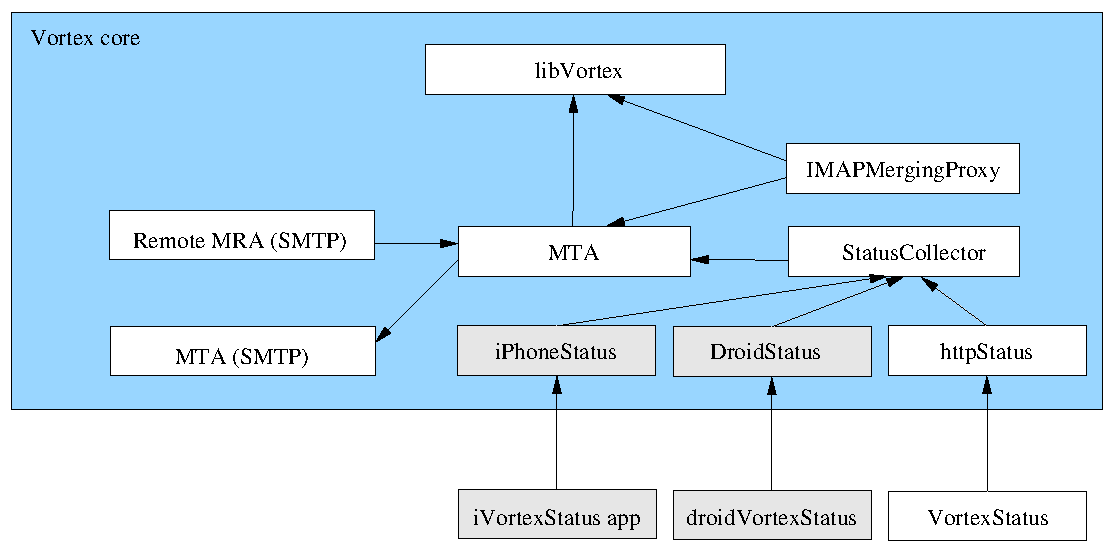
\includegraphics[width=\columnwidth]{inc/VortexModules}
	\caption{Overview of the Vortex modules}
	\label{fig:vortexModules}
\end{figure}

\section{Protocol Description}
\section{Accounting}
\section{Message Flows}

\section{Considerations for Building Messages}
In a worst case scenario we assume that an adverser is controlling most of the network utilized for anonymisation. While this is not nessessarily a problem (as pointed out earlier) it allows an adverser to track a message while agents are being used under his control. So for simplicity and as a worst case assumption we always assume that an adverser has perfect knowledge of an associated message flow. This is however a worst case scenario. One missing agent disconnects the whole chain and as messages are not traceable in size.

\subsection{Ephemeral identities}
\fxfatal{expiring ephemeral identities shold not only be replaced after their expiration but anytime during the livetime}
\subsection{Timing of messages}
\fxfatal{add content here}

\subsection{Building Diagnostic Paths}
\fxfatal{add content here}

\subsubsection{Implicit Diagnostic}
\fxfatal{Add comments about messages splitting and returning to sender}

\subsubsection{Automatic Explicit Diagnostic}
\fxfatal{Add comments about error and diagnosis messages officially spliting of messages}

\subsubsection{On-Demand Explicit Diagnostic}
\fxfatal{Add comments about normal, error, and diagnosis messages beeing picked up by a routing block}

\section{Considerations for Routing Messages}
\subsection{Time of sending}
Messages should always be sent timewise nearby other messages. This means that the best moment for sending a message in a ready queue is at a time when sending of other messages is due. However no optimisation should be done to send as many messages as possible at the same time. this would lead to a forseeable behaviour of the routing layer and thus to misusable behaviour.



\section{Real World Considerations}
This approach is heavily dependent of the transport protocol and builds on top a new obfuscating/routing layer. For this system to become a real peer-to-peer approach some additional quirks are required. A message-Vortex-Account needs always an active routing handler. This routing handler may be introduced by new server capabilities or by having a device handling the routing from the client side. For this reason we built a RaspberryPi appliance capable of connecting to one (or more) accounts fetching incomming mails, analysing them and reroute them if necessary. Although the system is designed to be run on a RaspberryPi the software might be installed to any Java capable client. The RaspberryPi is just an affordable lightweight device which offers all required capabilities.

\chapter{Security Analysis}
\fxfatal{add content here}

\chapter{Additional Considerations}
\fxfatal{add content here}

\section{Storage of Messages and queues}
The storage of messages sent though MessageVortex should be handled with great care. It seems on the first sight a good idea to merge all messages in a globally available storage such as the mail account of the receiving entity. However -- In doing so we would discover the message content to the providing party of a mail account. Since we handled the message with great care and tremendous costs up until this point it would be careless doing so. 

Storing them in a localized and receiving entity controlled storage is definitely a good idea but leaves security considerations like a backup possibly to an end user. This might be better but in effect a questionable decision. There is however a third option. By leaving the message unhandled on the last entity of the MessageVortex chain we may safely backup the data without disclosing the message content. Merging the content then dynamically through a specialized proxy would allow the user tu have a unified view on his without compromising the security.

\fxfatal{implemented in prototype?}

\section{Economy of transfer}
\fxfatal{Write something about wasting bandwidth}

\part{Discussion}
\fxfatal{add content here}

\chapter{Anonymity}
\fxfatal{add content here}

\section{Effects of anonymous communication on behaveour}
\fxfatal{add content}\cite{postmes2001social}


\backmatter
\appendix
\part{Appendix}
\makeatletter
\g@addto@macro\appendix{%
	\renewcommand*{\chapterformat}{%
		{\chapapp\nobreakspace\thechapter\autodot\enskip}%
	}
	\renewcommand*{\chaptermarkformat}{%
		{\chapapp\nobreakspace\thechapter\autodot\enskip}%
	}
	\let\oldaddcontentsline\addcontentsline
	\newcommand\hackedaddcontentsline[3]{\oldaddcontentsline{#1}{#2}{\chapapp\nobreakspace#3}}
	\let\oldchapter\chapter
	\renewcommand*\chapter[1]{%
		\let\addcontentsline\hackedaddcontentsline%
		\oldchapter{#1}%
		\let\addcontentsline\oldaddcontentsline%
	}
}
\makeatother
\onecolumn
\chapter{ASN.1 representation of the protocol\label{app:asnone}}
\lstinputlisting[language=ASN1, caption={ASN.1 representation of the protocol}, backgroundcolor=\color{gray!10}]{../app/asn.1/messageBlocks.asn} 
\twocolumn


\chapter{Glossary}

\begin{entry}
  \mainentry{adverser}{FIXME}
\end{entry}

\begin{entry}
  \mainentry{Agent}{FIXME}
\end{entry}

\begin{entry}
  \mainentry{EWS}{FIXME}
\end{entry}

\begin{entry}
  \mainentry{IMAP}{IMAP (currently IMAPv4) is a typical protocol to be used between a \defref{Client MRA} and a \defref{Remote MDA}. It has been specified in its current version in \cite{RFC3501}. The protocol is capable of fully maintaining a server based message store. This includes the capability of adding, modifying and deleting messages and folders of a mailstore. It does not include however sening mails to other destinations outside the server based store.}
\end{entry}

\begin{entry}
	\mainentry{Item of Interest (IoI)}{FIXME}
\end{entry}

\begin{entry}
  \mainentry{LMTP}{FIXME}
\end{entry}

\begin{entry}
  \mainentry{Local Mail Store}{A Local Mail Store offers a persistent store on a local non volatile memory in which messages are beeing stored. A store may be flat or structured (eg. supports folders). A Local Mail Store may be an authoritative store for mails or a ``Cache Only'' copy. It is typically not a queue.}
\end{entry}

\begin{entry}
  \mainentry{mail server admin}{FIXME}
\end{entry}

\begin{entry}
  \mainentry{MDA}{An MDA provides an uniform access to a \defref{Local Mail Store}.}
  \subentry{Remote MDA}{A Remote MDA is typically supporting a specific access protocol to access the data stored within a \defref{Local Mail Store} .}
  \subentry{Local MDA}{A Local MDA is typically giving local applications access to a server store. This may be done thru an API, a named socket or similar mechanisms.}
\end{entry}

\begin{entry}
  \mainentry{MRA}{A Mail receiving Agent. This agent receives mails from a agent. Depending on the used protocol two subtypes of MRAs are available.}
  \subentry{Client MRA}{A client MRA picks up mails in the server mail storage from a remote MDA. Client MRAs usually connect thru a standard protocol which was designed for client access. Examples for such protocols are \defref{POP} or \defref{IMAP}}
  \subentry{Server MRA}{Unlike a Client MRA a server MRA listens passively for incomming connections and forwardes received Messages to a MTA for delivery and routing. A typical protocol supported by an Server MRA is \defref{SMTP}}
\end{entry}

\begin{entry}
  \mainentry{MS-OXMAPIHTTP}{FIXME}
\end{entry}

\begin{entry}
  \mainentry{MSA}{A Mail Sending Agent. This agent sends mails to a \defref{Server MRA}. }
\end{entry}

\begin{entry}
  \mainentry{MTA}{A Mail Transfer Agent. This transfer agent routes mails between other components. Typically  an MTA receives mails from an MRA and forwardes them to a MDA or MSA. The main task of a MTA is to provide reliable queues and solid track of all mails as long as they are not forwarded to another MTA or local storage.}
\end{entry}

\begin{entry}
  \mainentry{MTS}{A Mail Transfer Service. This is a set of agents which provide the functionallity tor send and receive Messages and forward them to a local or remote store.}
\end{entry}

\begin{entry}
  \mainentry{MSS}{A Mail Storage Service. This is a set of agents providing a reliable store for local mail accounts. It also provides Interfacing which enables clients to access the users mail.}
\end{entry}

\begin{entry}
  \mainentry{MUA}{A Mail User Agent. This user agent reads mails from a local storage and allows a user to read existing mails, create and modify mails.}
\end{entry}

\begin{entry}
  \mainentry{Privacy}{From the Oxford English Dictionary: ``
    \begin{enumerate}
      \item The state or condition of beeing withdrawn from the society of others, or from the public intrest; seclusion. The state or condition of beeing alone, undisturbed, or free from public attention, as a matter of choice or right; freedom from interference or intrusion.
      \item Private or retired place; private apartments; places of retreat.
      \item Absence or avoidance of publicity or display; a condition approaching to secrecy or concealment. Keeping of a secret.
      \item A private matter, a secret; private or personal matters or relations; The private parts.
      \item Intimacy, confidential relations.
      \item The state of being privy to some act.
    \end{enumerate}''\cite[FIXME]{OXFORD}\\
    In this work privacy is related to definition two. Mails should be able to be handled as a virtual private place where no one knows who is talking to whom and about what or how frequent (except for directly involved people).
  }
\end{entry}

\begin{entry}
  \mainentry{POP}{POP (currently in version 3) is a typical protocol to be used between a \defref{Client MRA} and a \defref{Remote MDA}. Unlike \defref{IMAP} it is not able to maintain a mail store. Its sole purpose is to fetch and delete mails in a server based store. Modifying Mails or even handling a complex folder structure is not doable with POP}
\end{entry}

\begin{entry}
  \mainentry{Service}{FIXME}
\end{entry}

\begin{entry}
  \mainentry{SMTP}{SMTP is the most commonly used protocol for sending mails across the internet. In its current version it has been specified in \cite{RFC5321}.}
\end{entry}

\begin{entry}
  \mainentry{Storage}{A store to keep data. It is assumed to be temporary or persistent in its nature.}
\end{entry}

\begin{entry}
  \mainentry{user}{FIXME}
\end{entry}

\begin{entry}
  \mainentry{UBE}{FIXME}
\end{entry}

\chapter{Bibliography}
{
  \renewcommand*{\bibfont}{\small}
  \printbibliography[title={},heading=none]
}

% additional reference entries
\index{Mail transport|see {Message Transport}}

% add the index
\printindex

\begin{comment}
% just a trick to make TexNicCenter Bibliography working
\bibliography{mailvortex}
\bibliography{inc/bib/unclassified/Anonbib/anonbib}
\end{comment}



\begin{comment}
% Some Notes 
http://www.rfc-editor.org/pubprocess.html
RFC2223 Instructions to RFC Authors
RFC2119 BCP14 Key words for use in RFCs to Indicate Requirement Levels
RFC3979 BCP79 Intellectual Property Rights in IETF Technology
RFC5378 BCP78 Rights Contributors Provide to the IETF Trust


http://tex.stackexchange.com/questions/36307/formatting-back-references-in-bibliography
http://www.cs.columbia.edu/irt/software/l2x/ l2x -- conversion from LaTeX to other formats Version 1.13
http://ftp.gwdg.de/pub/ctan/support/l2x/
http://tools.ietf.org/tools/xml2rfc2

http://www.zisc.ethz.ch/events/2003-2011/ISC2006Slides/FederrathZISCTalk.pdf

Professorliste
Dr. Christoph Sprenger (Part I)
-Prof. David Basin
Gregory Demay
Peter Gazi
Dr. Srdjan Marinovic
Dr. Sasa Radomirovic
Dr. Ralf Sasse

T. Hoefler
A. Perrig 
-Dr. Jan Camenisch (Keine Berechtigung)

-Srdjan Capkun (Keine Kapazität)
-David Basin  (Keine Kapazität)
\end{comment}
\end{document}
